\chapter{Prototyping}

\section{Prototype \#1}

\subsection{Motivation}

The first prototype served as an initial experiment for investigating how technology might be used to give an audience new means of participating in a performance. My goal was to develop a simple system that featured a single user `performing' -- creating some sort of stimulating output. Multiple `audience members' would then be given the ability to collectively contribute to this output in some way, illustrating a slight shift from presentational to participatory. Ultimately, testing the prototype with users would allow me to observe how both the performer and audience members responded to these adjustments to their roles. I also hoped to establish a hardware and software framework upon which future prototypes could be easily built.
% It was designed for a colloquium -- to stimulate discussion

While the focus of this thesis is on rock performances, it was decided that recruiting a rock band would not be necessary for this early, small-scale experiment. I felt that a VJ performance would be suitable. VJing is the real-time creation or manipulation of visuals, which are typically projected to accompany music. Thus, the performing user would be controlling projected visuals, and the audience members would be able to manipulate some aspect of them. Having this collective output clearly displayed on one screen would provide the performer and audience members with clear feedback from their inputs and allow for straightforward observations of their interactions.
% Justification for VJ can come from analysis of ethnography; decision that I'll be focusing on visuals and not sound

Some design concepts were inspired by theory introduced in Chapter 2. The system was modelled after the ``core" and ``elaboration" roles outlined by Turino (2008). The performer -- the core role -- would be responsible for keeping the performance on track and have the most influence on the visuals. On the other hand, audience members -- elaboration roles -- would have less responsibility along with a lesser influence. In explaining presentational and participatory performances, Turino also states that it is not uncommon for a performer to shift between the two forms throughout one performance. To reflect this, I chose to include a feature allowing the performer to effectively `mute' input from the audience and take full control of the output.

% Background:
% Auslander, 1999: Communities are formed based on how the audience interacts, with no dependence on the spectacle at hand
% Turino, 2008:
% * Artists can shift between participatory and presentational performance
% * Different roles of different difficult allow for everyone to feel welcome and achieve flow. "Core" and "elaboration" roles cater to advanced and non-advanced performers respectively.
% * Open form: Basic motives repeated over and over. Easy for newcomers to join in. "Security in constancy." Can facilitate flow.
% * Hall: Repetition can increase intensity. Synchronicity comforts people.
% * Wide tuning, loud volumes, and overlapping textures provide a ``cloaking function'' that makes people more comfortable participating
% * Virtuosic solos are not common
% * Some participatory performances are sequential -- everyone gets a turn (e.g. Karaoke)
% Kelly, 2007: Displaying clips and themes from her music videos at a Madonna concert creates feelings of a "shared past" in the audience. (How might we create instead a "shared present"?)
% Small, 1998: Performers dressing in uniform are separating themselves and their responsibilities
% Davidson, 1997:
% * Performance etiquette is usually formed by crowd mentality, following the majority
% * Performers pick up information from the audience's broad and specific behaviours
% * Visuals help audiences read the performer's intentions
% Sexton, 2007: Simple synchronous interactions in sound art projects left users with little to explore, resulting in a "flat" experience
% Jourdain, 1997: We move to music in order to "represent" it. This also amplifies, resonates the musical experience.
% Levitin, 2006:
% * "In every society of which we're aware, music and dance are inseparable." Ancient music was based on rhythm and movement. Combining rhythm and melody bridges our cerebellum and cerebral cortex.
% * Ties between music and movement have only been minimized in the last 100 years
% Kelly, 2007: Technology incorporated into a show can either be addressed as part of the show or hidden and made illusory
% Maynes-Aminzade, 2002:
% * Computer vision: Movement-based control were intuitive, but camera required frequent calibration
% * Beach ball: Using a single beach ball as an input was also intuitive, but it only involved a few people at a time
% * Laser pointers: Gave everyone an individual cursor, but got chaotic once more and more people joined
% * Recommendations: Focus on compelling activity over impressive technology. Not everyone must be sensed as long as they feel involved. The control mechanism should be obvious or the users will give up. Make the activity emotionally engaging. Emphasize cooperation.
% Ulyate, 2001:
% * Design guidelines:
% * * Encourage and reward movement
% * * Feedback should be immediate, obvious, and meaningful in the context of the space
% * * No instruction or thinking should be required
% * * Responsiveness is more important than aesthetics
% * *  Modularity is key
% * Lessons learned:
% * * Full-body movement is most satisfying
% * * Form of the object determines how users interact
% * * A practical system is distributed and scalable
% * * Find balance between freedom and constraint
% * * Users will always find a way to create unwanted outputs
% * * Simple, instant gratification is important for feedback
% Barkhuus, 2008:
% * Inputs based on already-present behaviour lead to intuitive systems
% * Don't focus on employing cutting edge technology
% * Events should not rely on the success of the technology
% * Immediate visual or aural feedback is key
% Tseng, 2012: Being excluded from the interaction did not lessen enjoyment of the show
% Reeves, 2010:
% * "Intra-crowd interaction" is a common phenomena to exploit
% * Many actions "snowball" and overtake crowds; highly visible/audible actions promote this
% * People on the fringes of the crowd interact, but there is latency
% * Every crowd is different; designs should reflect the environment
% Gates, 2006: Technologies should reflect the performer's art and not be a burden on them

\subsection{Development}

The first step in realizing this initial prototype was deciding on the hardware and software that would be used. Wii video game controllers have an abundance of sensors: they contain eleven digital buttons, an infrared sensor, an accelerometer, and a gyroscope (in the newer Wii Remote Plus models), and all of this data can be sent wirelessly to a receiver via Bluetooth. In addition to these affordances, due to the console's popularity, the Wii controller is also something that many people have already used before. With these considerations, I decided that the Wii controller was a suitable input device for my experiment. For my purposes, the easiest way to process the controllers' data was using a combination of two software packages -- OSCulator\footnote{\url{http://www.osculator.net}} and Max\footnote{\url{http://cycling74.com}}. OSCulator allows for communication between devices and audio or video software using the Open Sound Control (OSC) protocol\footnote{\url{http://opensoundcontrol.org}}. Fortunately, this software is also specifically designed to communicate with the Wii controller. It can display live data from each sensor as well as activate the controller's LEDs and rumble motor. The data can then be sent to Max, a visual programming environment that is especially useful for handling multimedia. Countless objects can be incorporated into a Max program (called a `patcher') to manipulate numbers, audio signals, and video clips. Max is commonly used by musicians and video artists to create highly customized and interactive programs.

\begin{figure}[t]
	\centering

	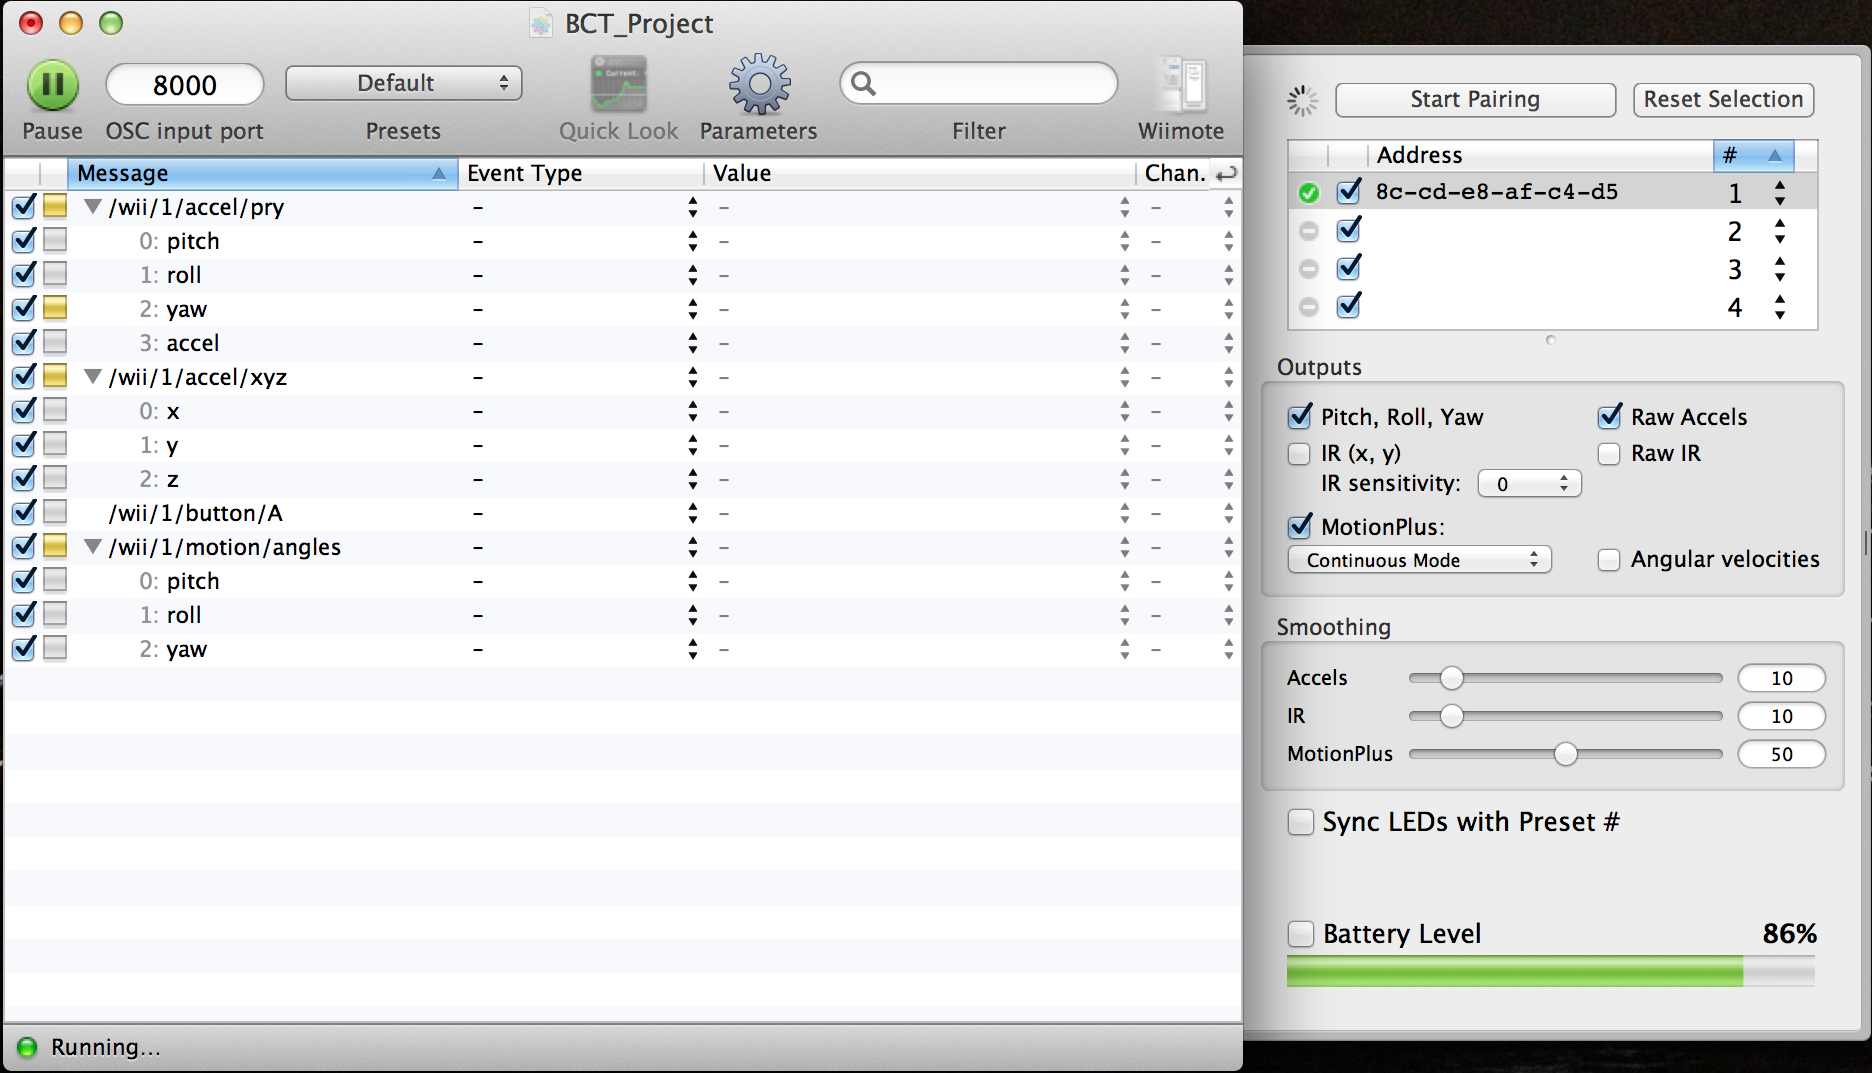
\includegraphics[height=0.4\textwidth]{osculator_1.png}
	\caption{OSCulator software receiving data from one Wii controller}

	\label{prototyping1.1}
\end{figure}

Syncing the Wii controller with OSCulator was simple, and I was immediately able to view movement and push-button data from my controller (see Figure \ref{prototyping1.1}). Next, I tested the limit of how many Wii controllers would be able to connect to my computer using the current setup. Since my thesis aims to give every member of an audience a new way to participate, this number would ideally be limitless. With Bluetooth technology, unfortunately, one master device (my computer) can only connect to a maximum of seven slave devices (Wii controllers). However, for the purposes of this prototype, I felt that seven controllers would be acceptable. A Max patcher was created to display push-button data from multiple Wii controllers. All seven were synced with no issues, and the program worked as expected (see Figure \ref{prototyping1.2}).

\begin{figure}[t]
	\centering

	\subfloat[Wii controllers]{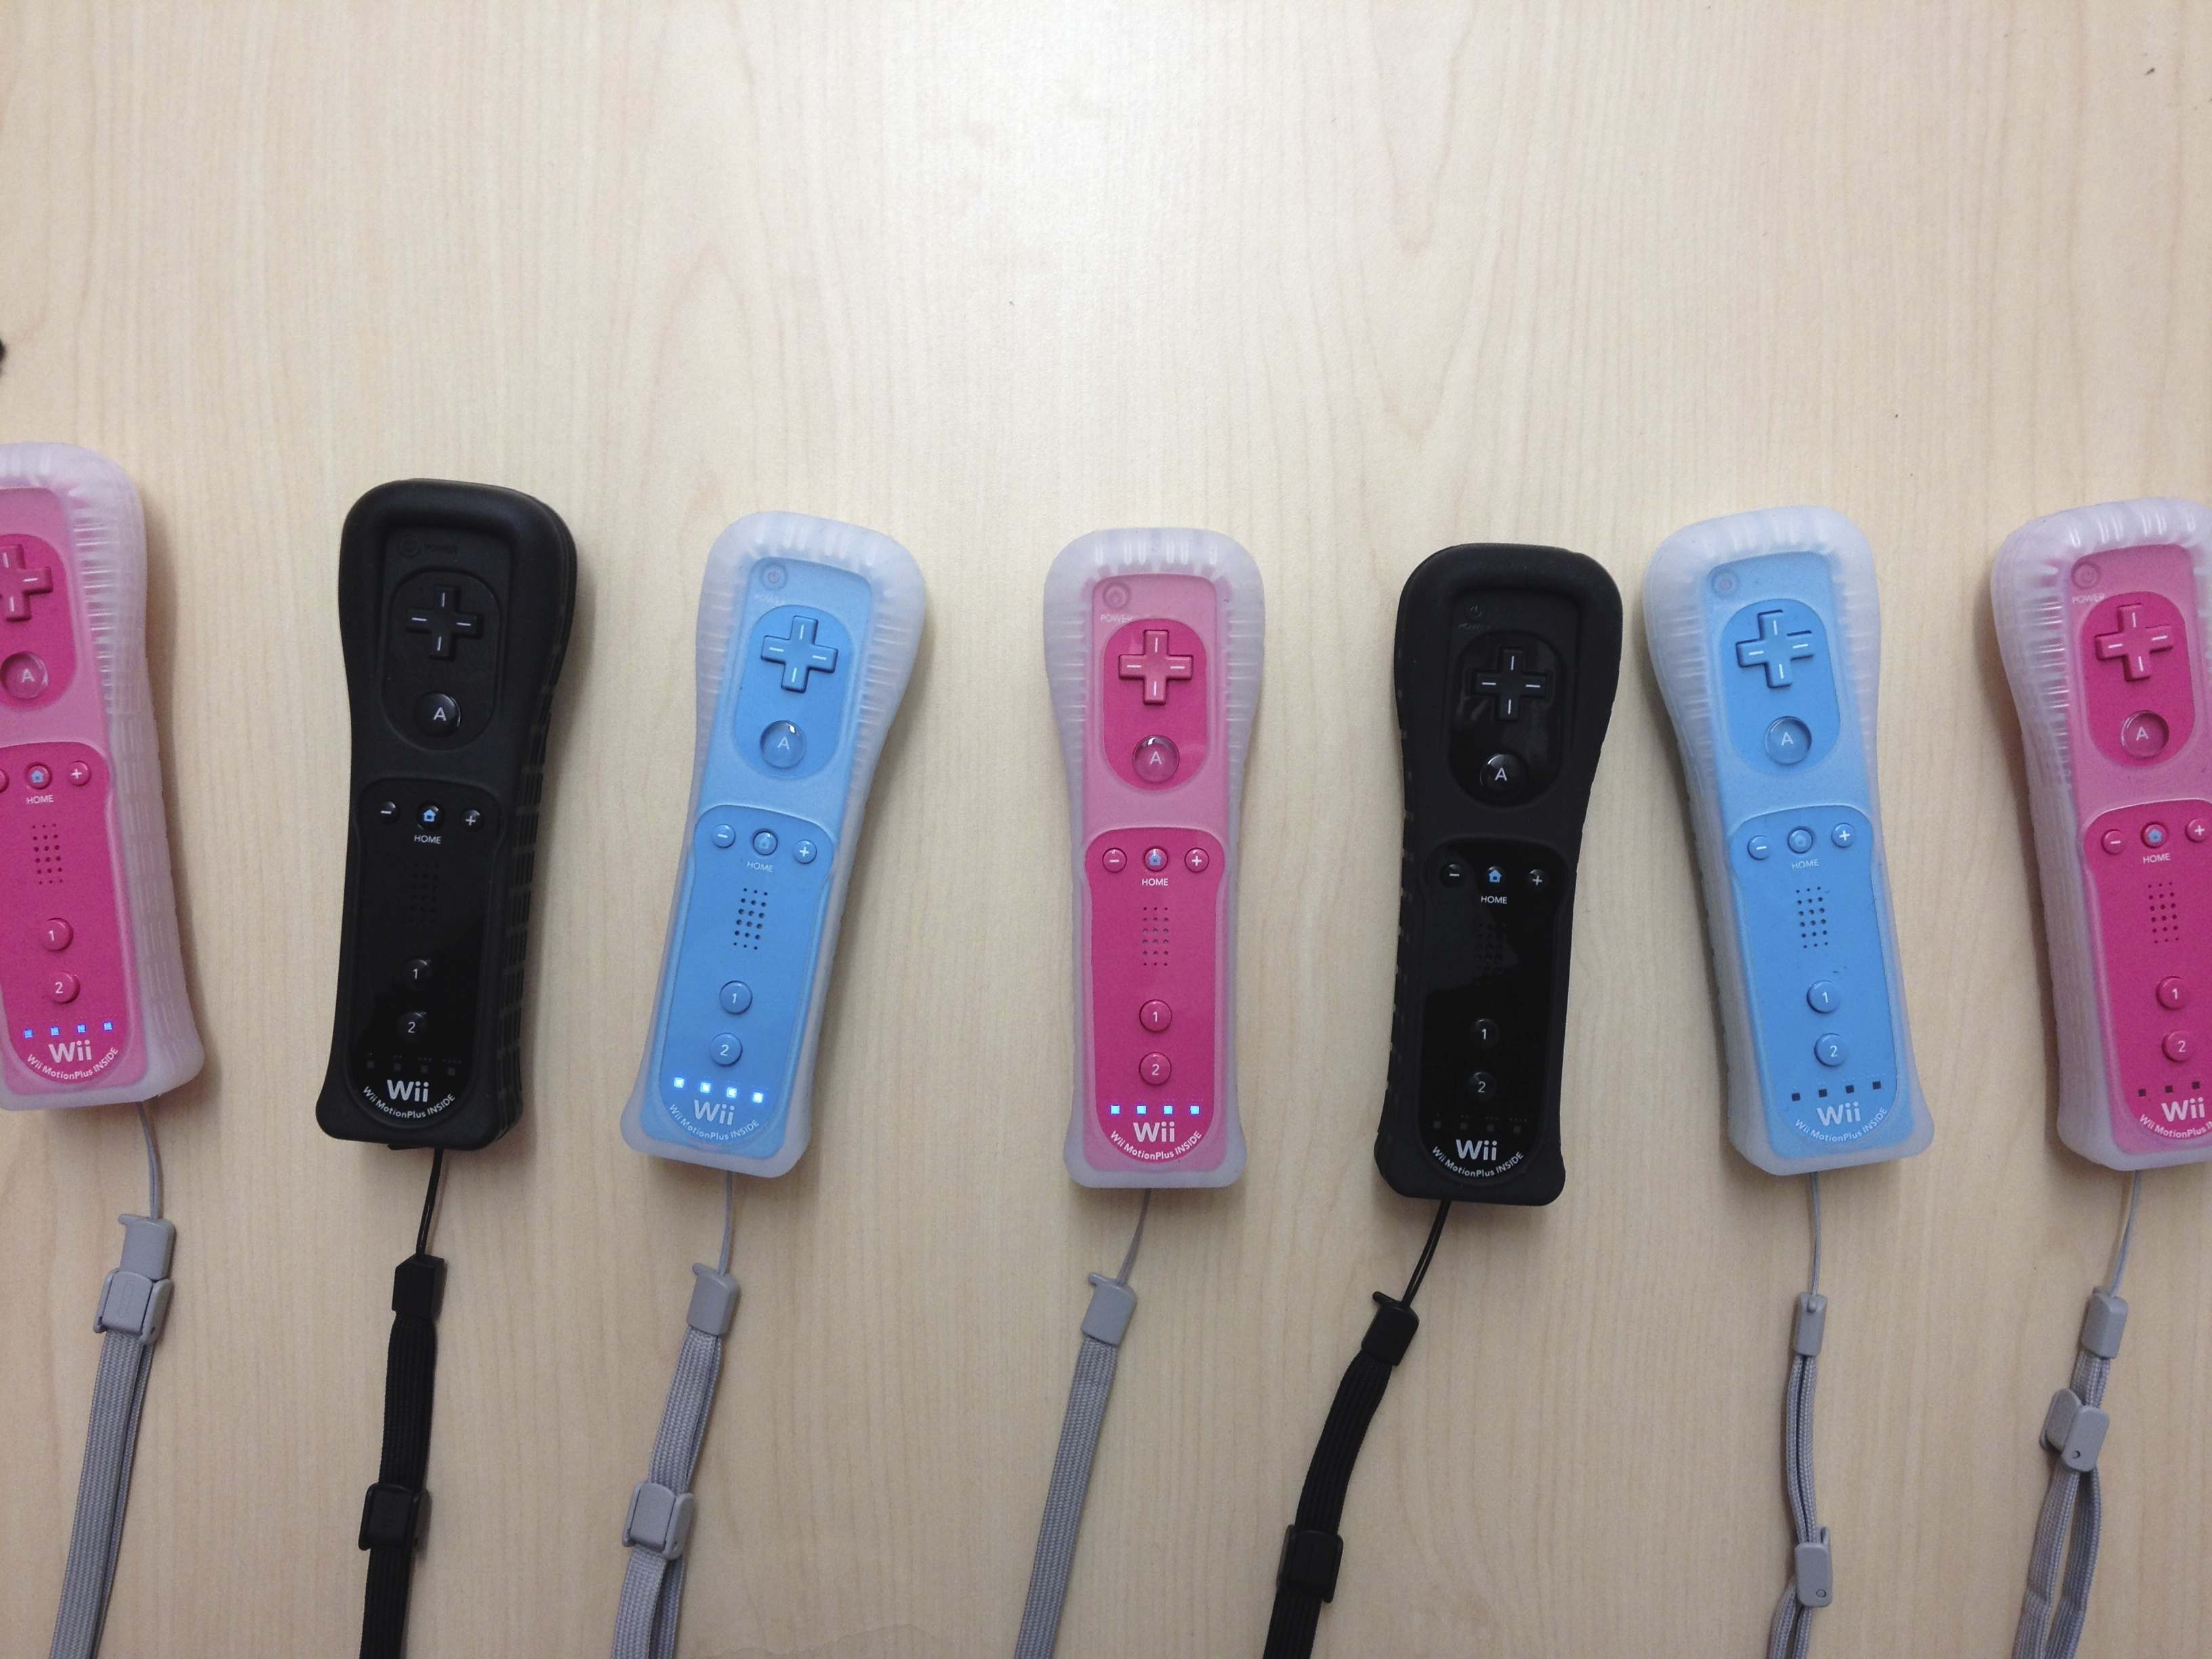
\includegraphics[height=0.32\textwidth]{wiimotes.jpg}}
	\hspace{0.1cm}
	\subfloat[Max patcher: The LED objects turn yellow when the A button is pressed on their assigned controller]{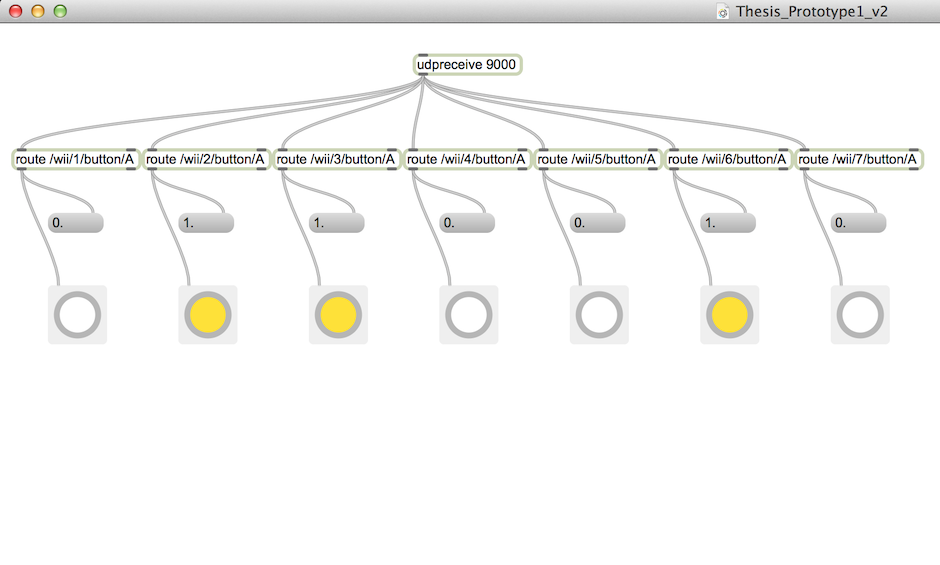
\includegraphics[height=0.32\textwidth]{multi_wii.png}}
	\caption{Testing simultaneous input from seven Wii controllers}

	\label{prototyping1.2}
\end{figure}

My next task was to create the VJ system. After experimenting with a multitude of video effects objects in Max, I created a basic program. The system is built around two short video loops that can be mixed together and modified. Users can crossfade between the two videos using the controller's Left and Right buttons. The resulting image can be rotated by rotating the controller sideways. Pixelation can be increased or decreased by increasing or decreasing the controller's incline. Finally, holding and releasing the A button enables and disables a motion blur effect. An important part of programming this patcher was mapping controller input to the effects controls. Values had to be carefully scaled and clipped in order for users' movements to translate naturally to the effect they control. I also carefully selected the source video such that the effects of users' actions would be clear; a black and white clip of one person dancing and a colour clip of multiple people dancing seemed to offer sufficient contrast (see Figure \ref{prototyping1.3}). The resultant patcher is pictured in Figure \ref{prototyping1.4}.

\begin{figure}[t]
	\centering

	\subfloat[Black and white]{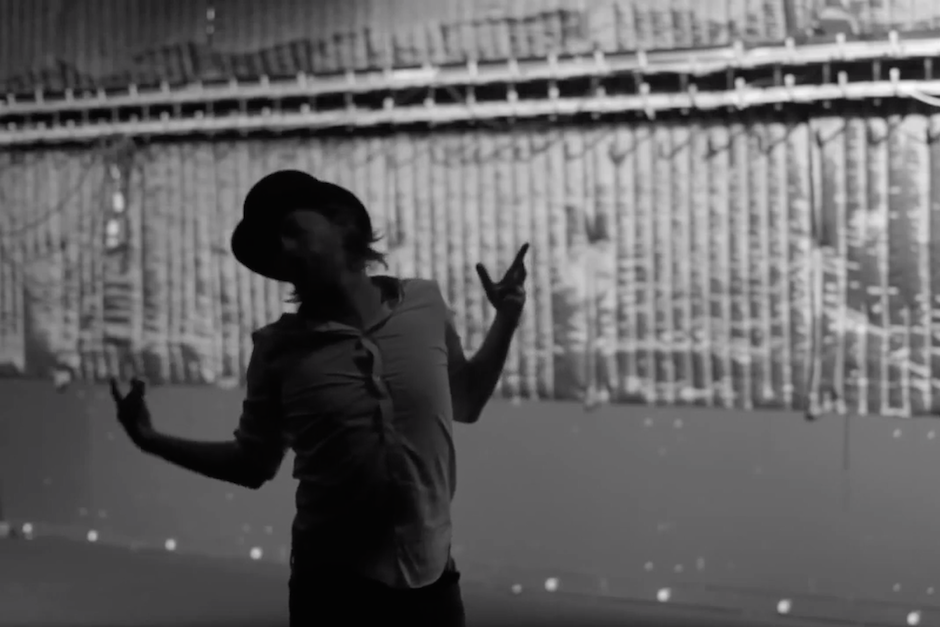
\includegraphics[height=0.32\textwidth]{vid_1.png}}
	\hspace{0.1cm}
	\subfloat[Colour]{\includegraphics[height=0.32\textwidth]{vid_2.png}}
	\caption{Stills from the two clips used in the prototype}

	\label{prototyping1.3}
\end{figure}

\begin{figure}[t]
	\centering

	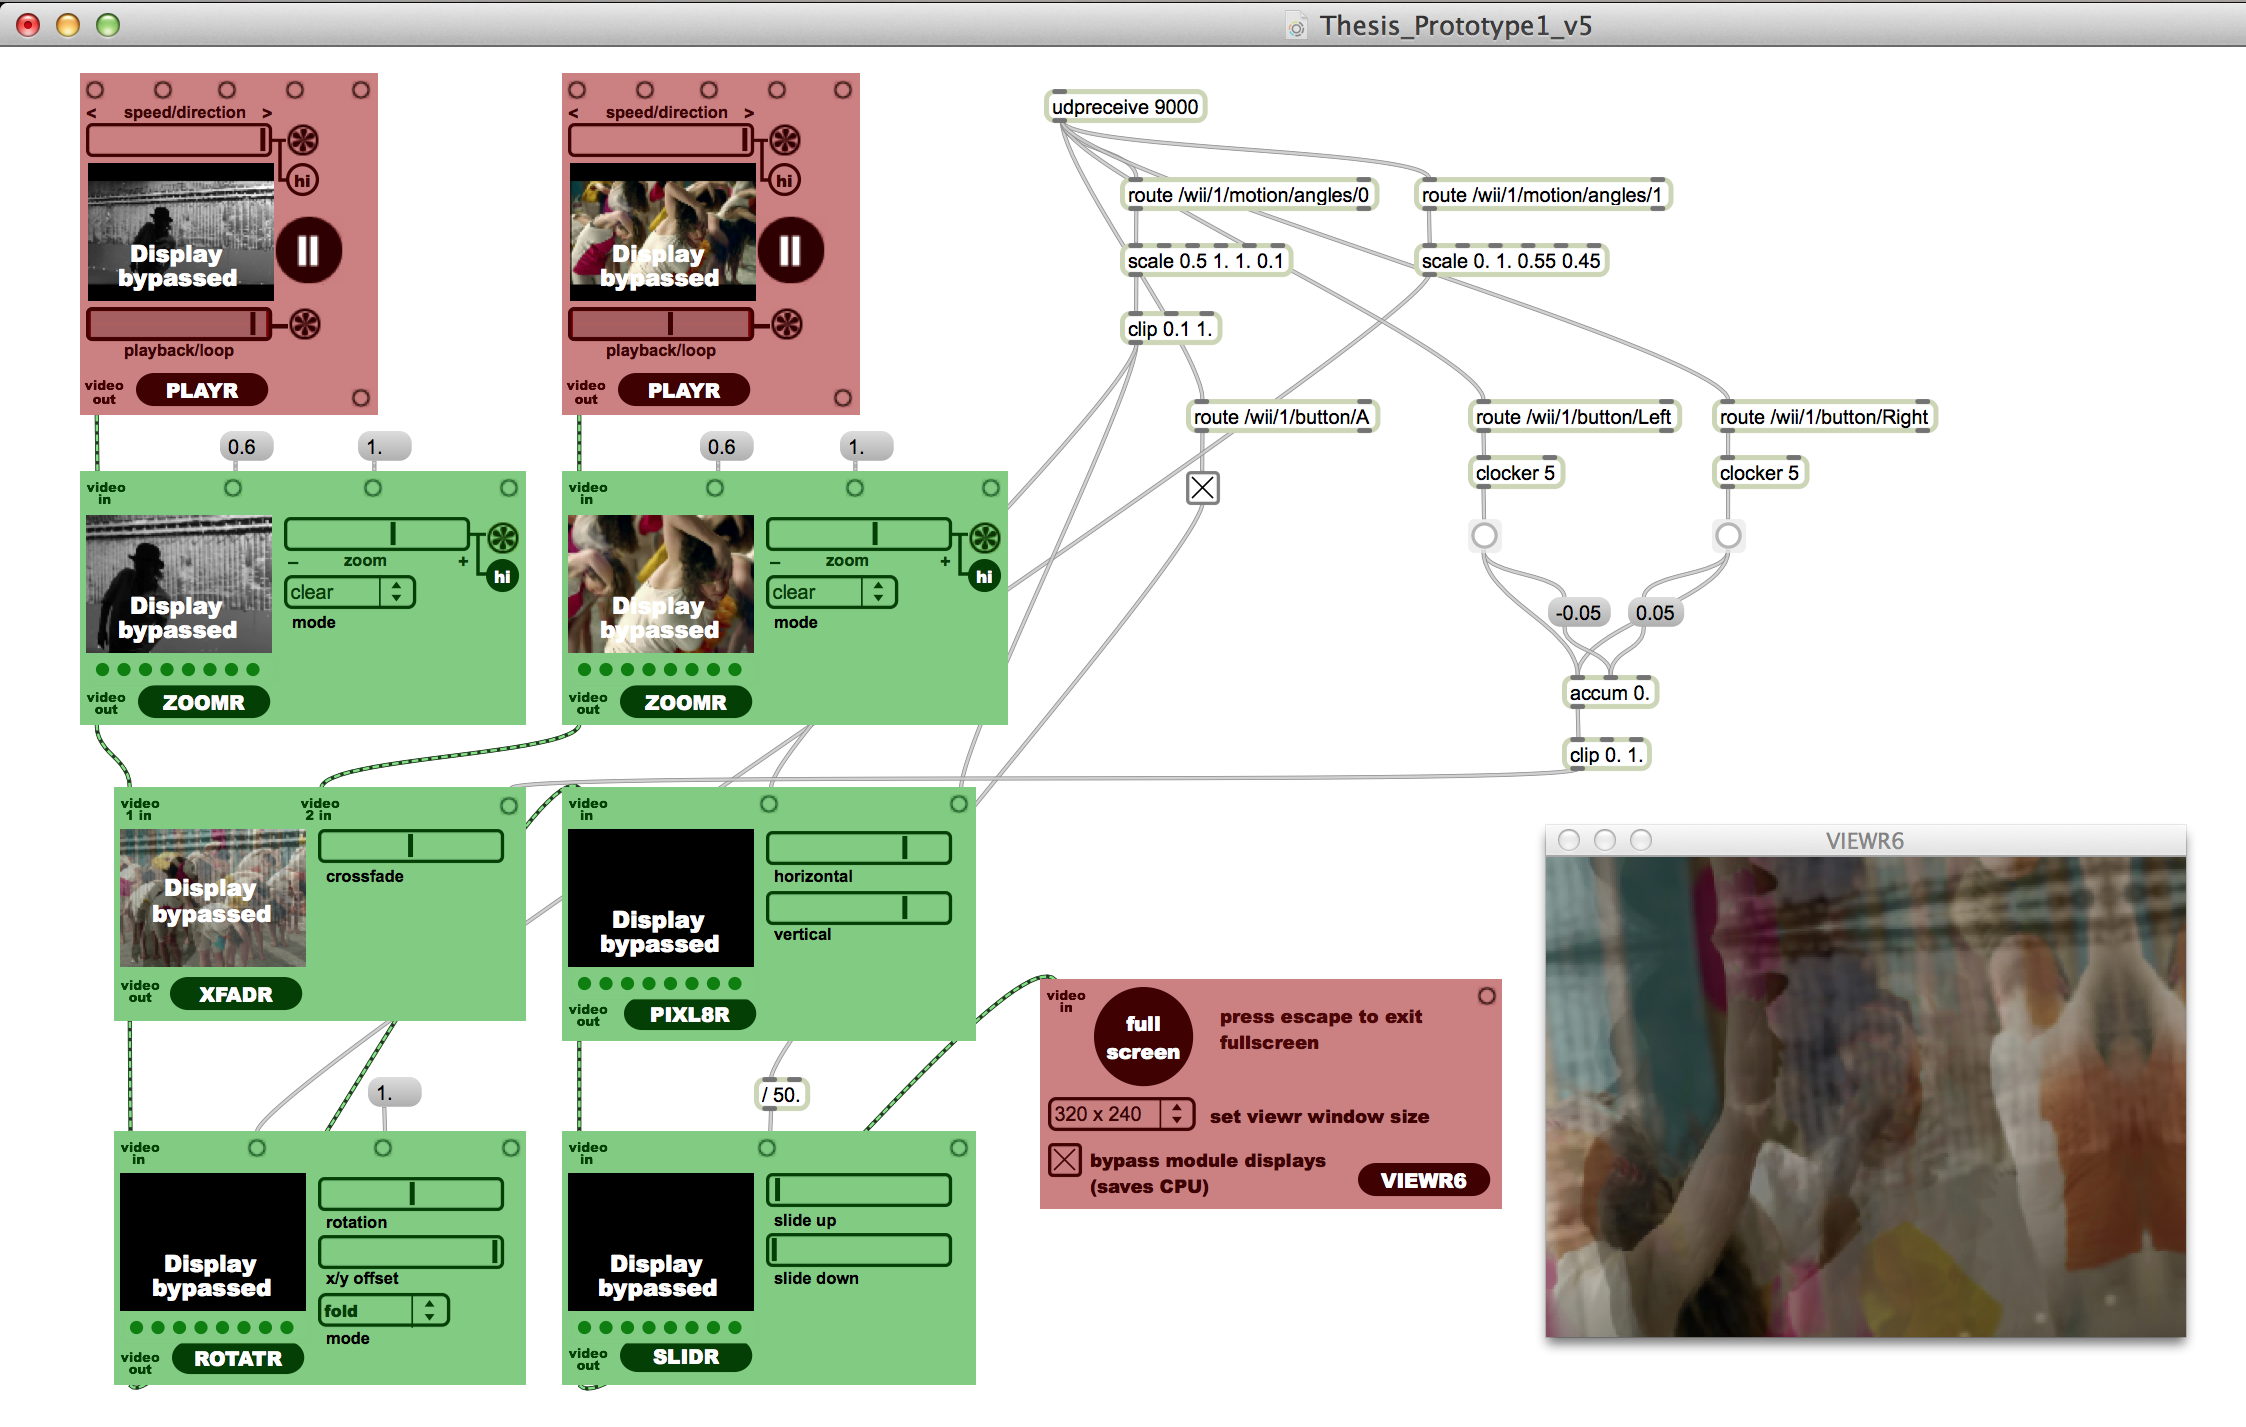
\includegraphics[height=0.4\textwidth]{wii_vj.png}
	\caption{Wii controller VJ system}

	\label{prototyping1.4}
\end{figure}

With the details of the performance in place, the next step was selecting which aspect would be controlled by the audience. It seemed most straightforward to give them control over the crossfader effect. This presents audience members with a simple binary decision -- do you want to see more of the black and white video or the colour video? By pressing and holding the Left or Right buttons on their controllers, users can effectively vote on which dominates the screen. In this case, if more people are holding the Left button than the Right, the black and white video will gradually become more prominent than the coloured video. Thus, while the performer retains precise control over multiple combinable effects (rotation, pixelation, motion blur), the collective audience can progressively alter the tone of the visuals. This reflects Turino's (2008) core and elaboration roles, respectively.

The last feature of this VJ system reflects another of Turino's (2008) assertions -- that performers often shift between presentational and participatory performance. In response to this, I provided the performing user with a mute function. By pressing the controller's B button, the performer can disable the audience members' controllers, moving control of the crossfader from the audience to the performer. The B button is essentially an on/off switch for audience participation.

The completed first prototype is illustrated in Figure \ref{prototyping1.5}, in the form of both a diagram and the final Max patcher.
% Make a diagram to illustrate the final product

\begin{figure}[t]
	\centering

	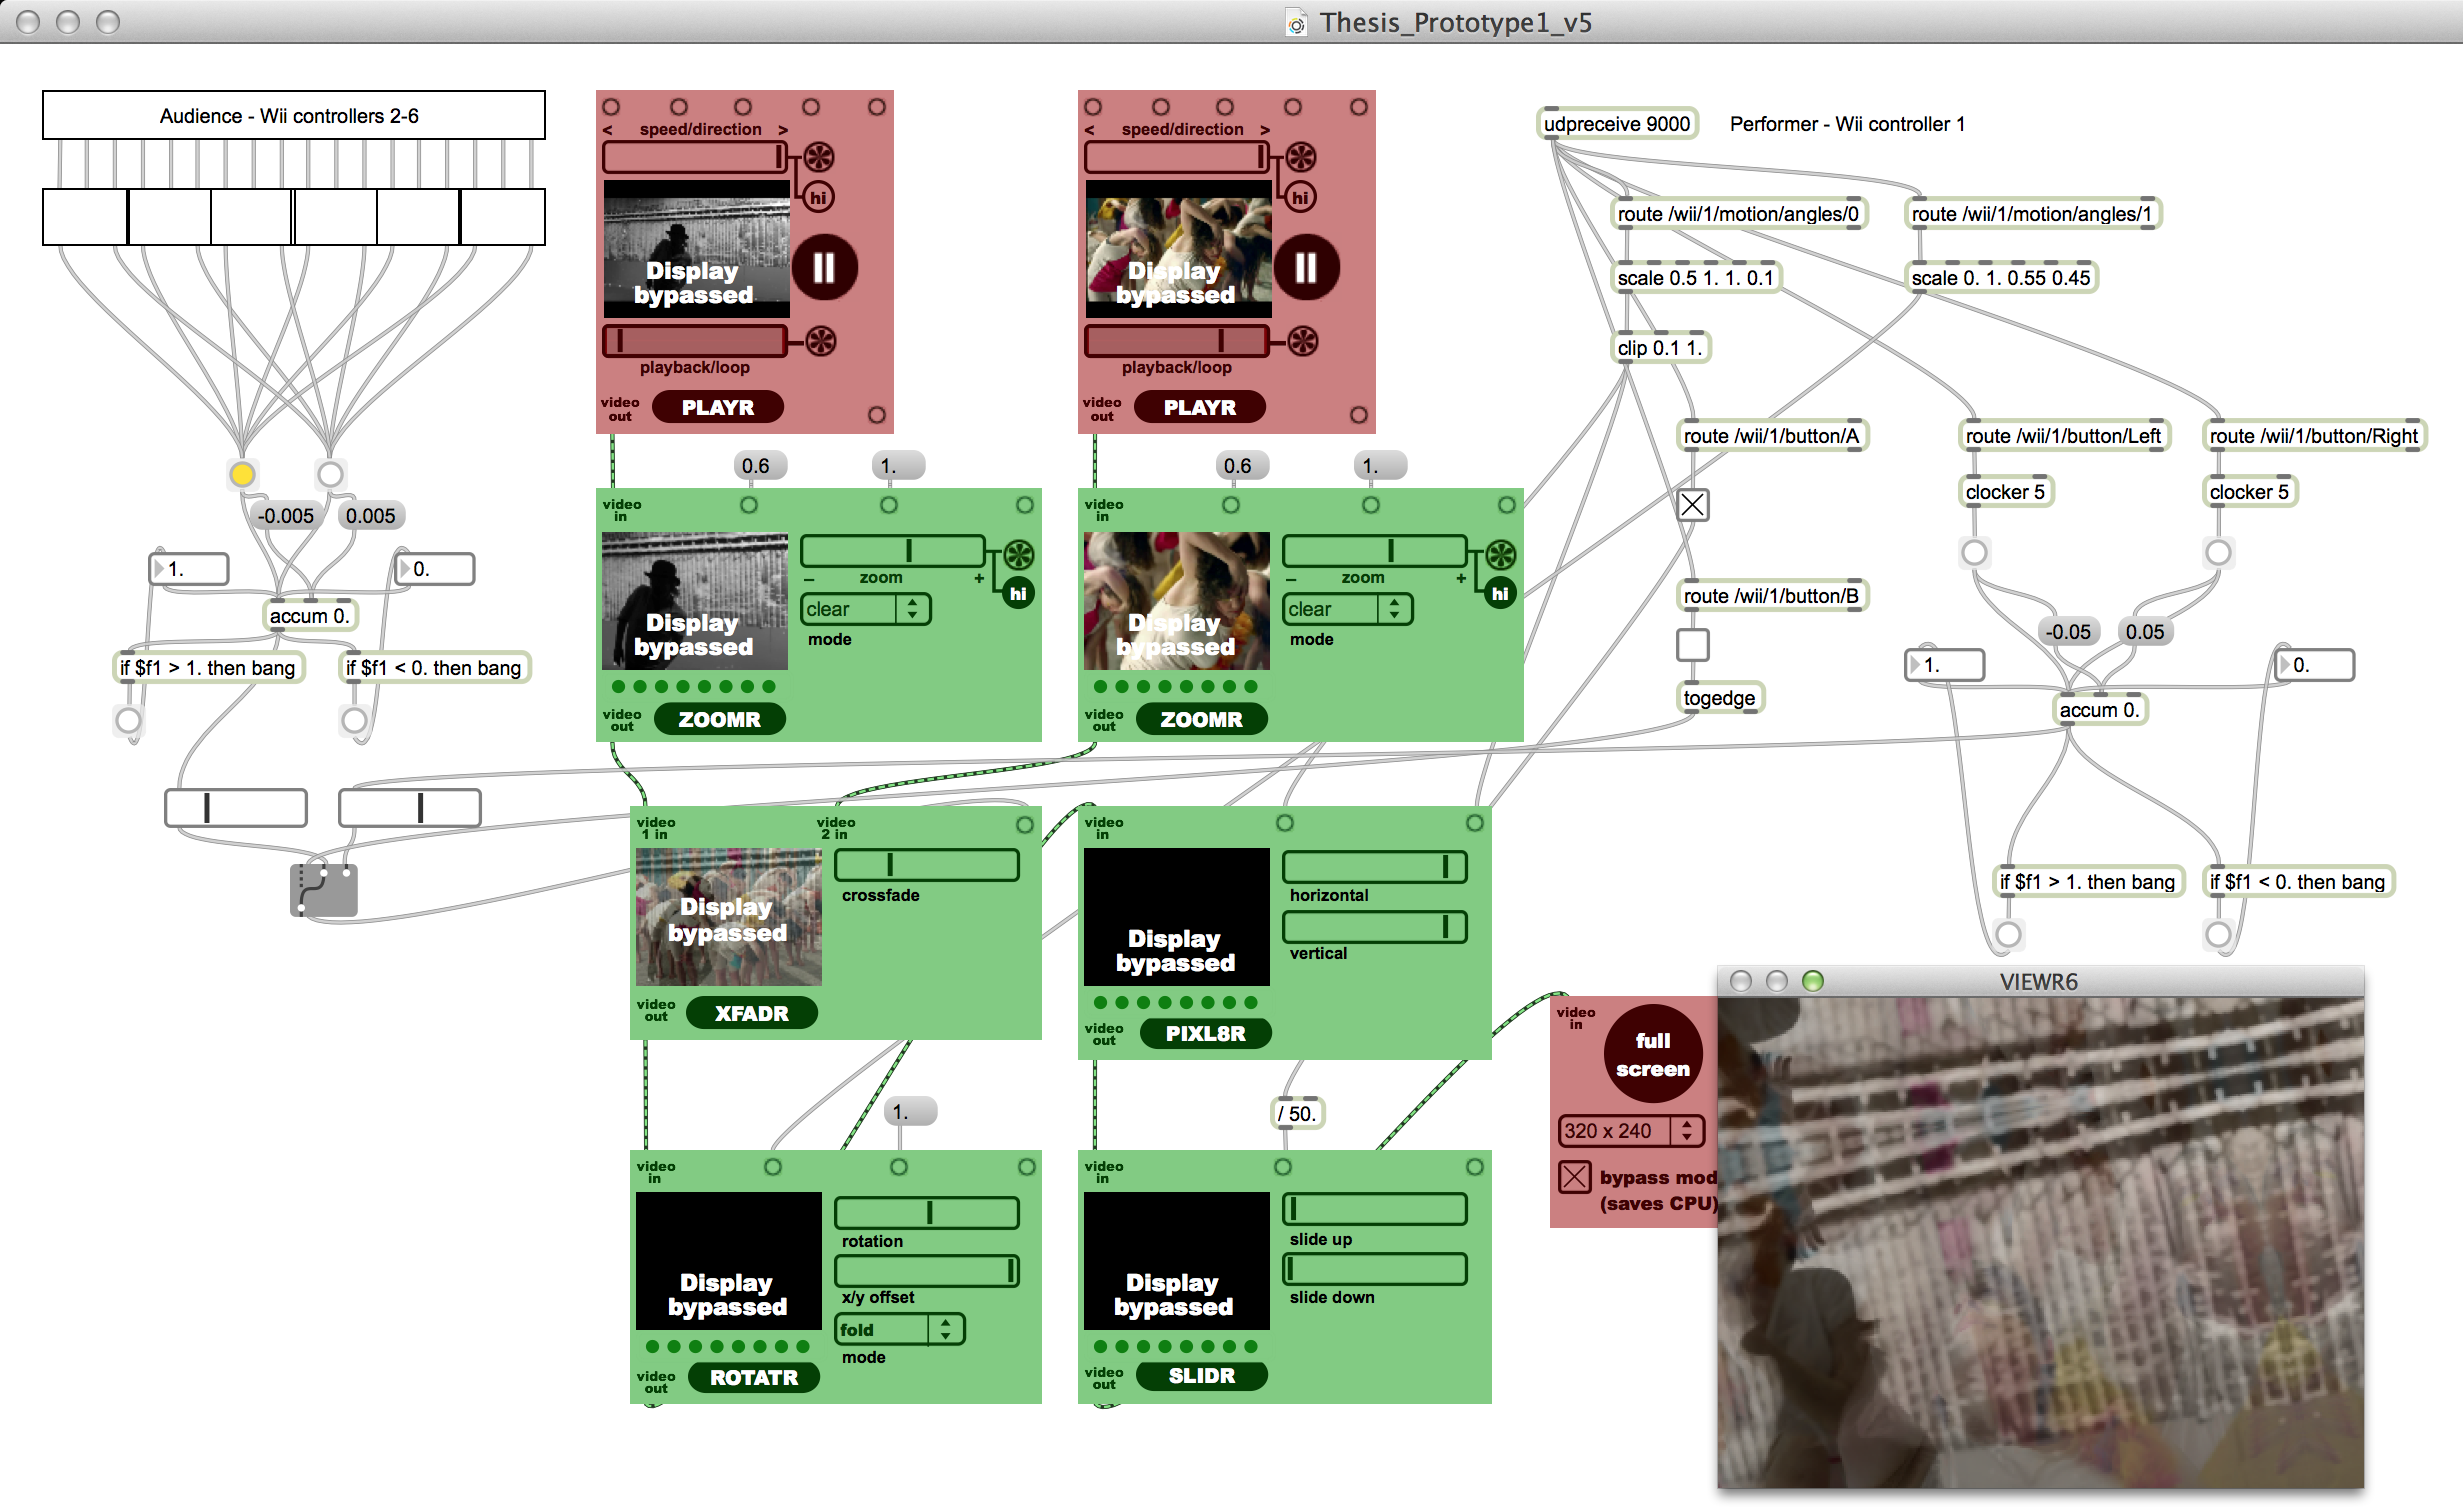
\includegraphics[height=0.4\textwidth]{vj_and_audience.png}
	\caption{Prototype \#1 Max patcher}

	\label{prototyping1.5}
\end{figure}

\subsection{Testing}
% Explain the details of how participants were recruited, how data was collected, recorded, and processed/analyzed, and the timeline over which this process unfolded

Testing was conducted one time with a small group at a research colloquium. I observed user behaviour and received feedback from attendees. The participants were seven OCADU students. The experiment only lasted a few minutes. I explained the concept and controls. The performer had no problem using his controls to make interesting visual output. One participant led the group in first fading all the way to one video then all the way to the other. Nothing broke, and the group successfully made decisions and carried them collaboratively. The performer's mute button worked.

Context is important; experiments should be run at rock shows or in similar environments. Observers commented on the importance of feedback. They asked if this sort of system should be goal oriented; if not, would the users somehow turn it into a game anyways? They considered the task of representing every individual. Will every single audience member be able to interact? What happens to those who are not included? They referenced `the wave' -- there's a flow, a rhythm; the outcome is greater than the sum of its parts; participants know when it's their turn to input...

\subsection{Analysis}

% Thoughts:
% * Two buttons: Improving on binary input (cheering, the lighter). Taking audience input from digital towards analog.
% * If we ask the audience to make a decision, will it change throughout the show? (Later: Yes/No vs How; i.e. Prototype 1 vs 3)
% * Mute: When should the audience have control?
% * Goal oriented? Should the users be trying to achieve something? Will they find a way to turn it into a game regardless?
% * What about spectators who are not participants? Tseng et al. indicate those left out can still get enjoyment. Heck, even watching videos of the precedent projects can be exhilarating.


\section{Prototype \#2}

This chapter covers the development of the second prototype. I explain the design goals, the creation process, and the user testing that was carried out. The chapter closes with a discussion on the significance of the prototype.

\subsection{Motivation}

This prototype's purpose was to explore possible input mechanisms for audience members. Through user testing, I hoped to identify which were intuitive, which were most natural and meaningful to perform as a group, and which afforded accurate collaborative control. From the start, it was clear that body movement would be more a fitting input than something like button pressing. Users find movement-based interactions more satisfying (Ulyate \& Biancardi, 2001); furthermore, there are apparent subconscious ties that link music and movement (Jourdain, 1997; Levitin, 2006), making this a natural form of input for a live music environment. In designing their audience-interaction system, Barkhuus and Jorgensen (2008) found that movements based on already-present behaviour were especially effective input methods. Inspired by this recommendation, I created a list of common crowd behaviours to be incorporated in the system -- giving a thumbs up or thumbs down, swaying one's arms back and forth, clapping, doing `the wave' (also known as 'the Mexican wave'), holding a lighter in the air, and dancing. Researchers emphasize the importance of meaningful feedback in crowd-controlled systems (Ulyate \& Biancardi, 2001; Barkhuus \& Jorgensen, 2008), and this was also a recurring concern in the response to Prototype \#1. Thus, this prototype also allowed for exploration of different feedback methods. After receiving the opportunity to participate in an exhibition at OCAD University, I decided to design this prototype as an interactive installation. By inviting the exhibition attendees to test the various methods of input, I could observe the behaviours of a wide variety of users.

% Background:
% Auslander, 1999: Communities are formed based on how the audience interacts, with no dependence on the spectacle at hand
% Turino, 2008:
% * Artists can shift between participatory and presentational performance
% * Different roles of different difficult allow for everyone to feel welcome and achieve flow. "Core" and "elaboration" roles cater to advanced and non-advanced performers respectively.
% * Open form: Basic motives repeated over and over. Easy for newcomers to join in. "Security in constancy." Can facilitate flow.
% * Hall: Repetition can increase intensity. Synchronicity comforts people.
% * Wide tuning, loud volumes, and overlapping textures provide a ``cloaking function'' that makes people more comfortable participating
% * Virtuosic solos are not common
% * Some participatory performances are sequential -- everyone gets a turn (e.g. Karaoke)
% Kelly, 2007: Displaying clips and themes from her music videos at a Madonna concert creates feelings of a "shared past" in the audience. (How might we create instead a "shared present"?)
% Small, 1998: Performers dressing in uniform are separating themselves and their responsibilities
% Davidson, 1997:
% * Performance etiquette is usually formed by crowd mentality, following the majority
% * Performers pick up information from the audience's broad and specific behaviours
% * Visuals help audiences read the performer's intentions
% Sexton, 2007: Simple synchronous interactions in sound art projects left users with little to explore, resulting in a "flat" experience
% Jourdain, 1997: We move to music in order to "represent" it. This also amplifies, resonates the musical experience.
% Levitin, 2006:
% * "In every society of which we're aware, music and dance are inseparable." Ancient music was based on rhythm and movement. Combining rhythm and melody bridges our cerebellum and cerebral cortex.
% * Ties between music and movement have only been minimized in the last 100 years
% Kelly, 2007: Technology incorporated into a show can either be addressed as part of the show or hidden and made illusory
% Maynes-Aminzade, 2002:
% * Computer vision: Movement-based control were intuitive, but camera required frequent calibration
% * Beach ball: Using a single beach ball as an input was also intuitive, but it only involved a few people at a time
% * Laser pointers: Gave everyone an individual cursor, but got chaotic once more and more people joined
% * Recommendations: Focus on compelling activity over impressive technology. Not everyone must be sensed as long as they feel involved. The control mechanism should be obvious or the users will give up. Make the activity emotionally engaging. Emphasize cooperation.
% Ulyate, 2001:
% * Design guidelines:
% * * Encourage and reward movement
% * * Feedback should be immediate, obvious, and meaningful in the context of the space
% * * No instruction or thinking should be required
% * * Responsiveness is more important than aesthetics
% * *  Modularity is key
% * Lessons learned:
% * * Full-body movement is most satisfying
% * * Form of the object determines how users interact
% * * A practical system is distributed and scalable
% * * Find balance between freedom and constraint
% * * Users will always find a way to create unwanted outputs
% * * Simple, instant gratification is important for feedback
% Barkhuus, 2008:
% * Inputs based on already-present behaviour lead to intuitive systems
% * Don't focus on employing cutting edge technology
% * Events should not rely on the success of the technology
% * Immediate visual or aural feedback is key
% Tseng, 2012: Being excluded from the interaction did not lessen enjoyment of the show
% Reeves, 2010:
% * "Intra-crowd interaction" is a common phenomena to exploit
% * Many actions "snowball" and overtake crowds; highly visible/audible actions promote this
% * People on the fringes of the crowd interact, but there is latency
% * Every crowd is different; designs should reflect the environment
% Gates, 2006: Technologies should reflect the performer's art and not be a burden on them

\subsection{Development}

The first prototype provided a suitable framework for this experiment: I continued using multiple Wii controllers as input devices, and OSCulator was used to route the data to Max where it processed and represented visually. From here, I needed to be able to recognize when a user was performing one of the selected crowd behaviours. By pulling data from the controller's motion sensors, I was able to identify when the user was giving a thumbs up or down, swaying their arms left or right, clapping, or doing the wave. I incorporated simple visual feedback -- LED objects that light up when the user holds their thumb up or down or claps, sliders that follow arm movement when the user is swaying or doing the wave. Calibrating these required trial and error tests using different thresholds -- determining what amount of acceleration qualified as a clap, for instance. Figure \ref{prototyping2.1} shows the first iteration of this prototype.

\begin{figure}[t]
	\centering

	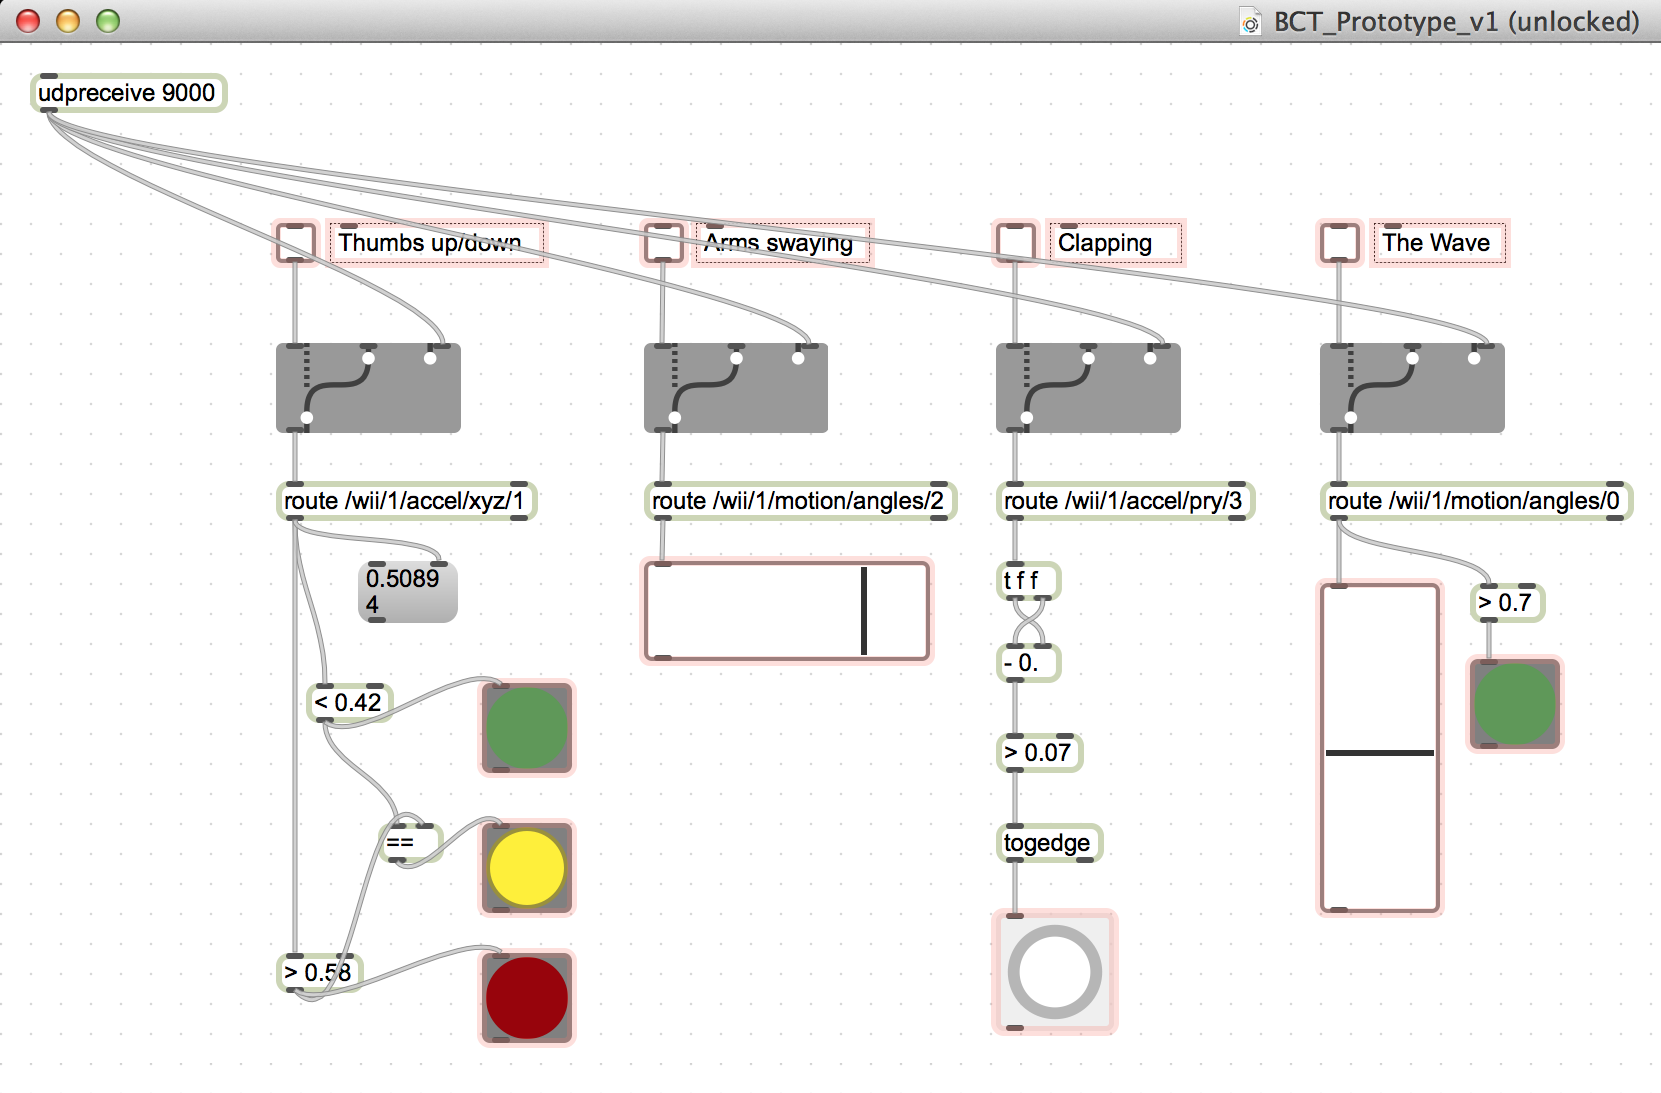
\includegraphics[height=0.4\textwidth]{wiimote_audience.png}
	\caption{Monitoring thumbs up/down, arm swaying, clapping, and the wave}

	\label{prototyping2.1}
\end{figure}

Next, I modularized the previous patcher and multiplied it sevenfold. The actions of seven users could now be monitored simultaneously. I developed new visualizations to reflect these multiple inputs, shown in Figure \ref{prototyping2.2}. Thumbs up/down mode simply displays how many users are holding their thumbs up and down. The wave mode shows the vertical position of each user's arms. I created two modes to detect clapping. The first displays seven LED objects that illuminate when each user claps, encouraging users to clap in sync. The second serves as a `clap-o-meter,' visualizing the collective clapping activity. Lastly, the swaying mode includes a slider to display the left-right movement of each user.

\iffalse
\begin{figure}[t]
	\centering

	\subfloat[Thumbs up/down]{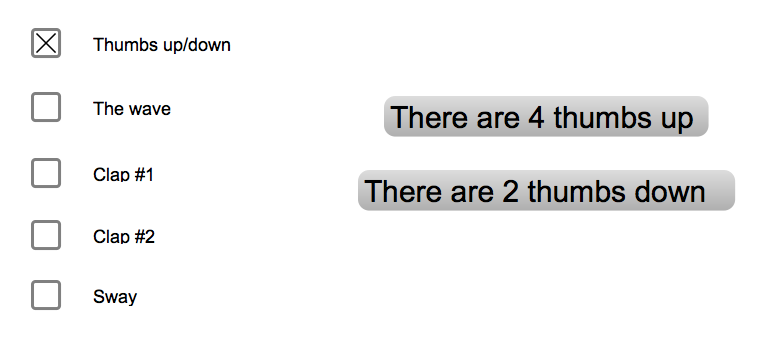
\includegraphics[height=0.2\textwidth]{thumbs.png}}
	\hspace{0.1cm}
	\subfloat[The wave]{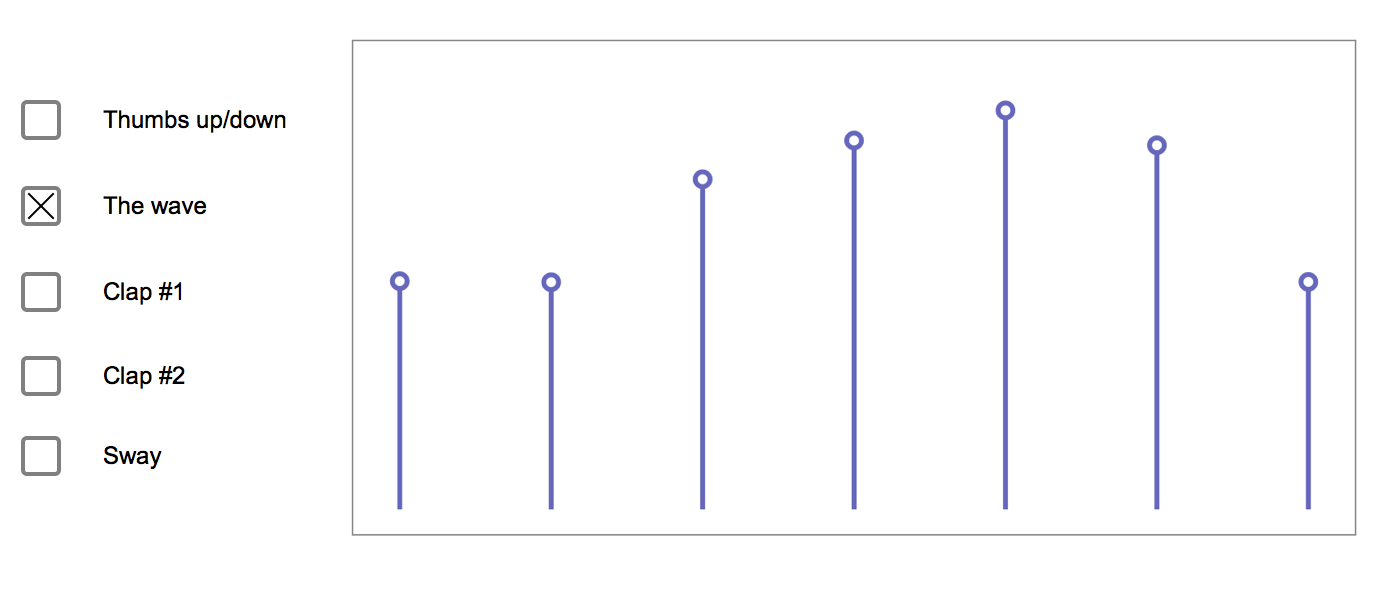
\includegraphics[height=0.2\textwidth]{wave.png}}	
	\hspace{0.1cm}
	\subfloat[Clapping]{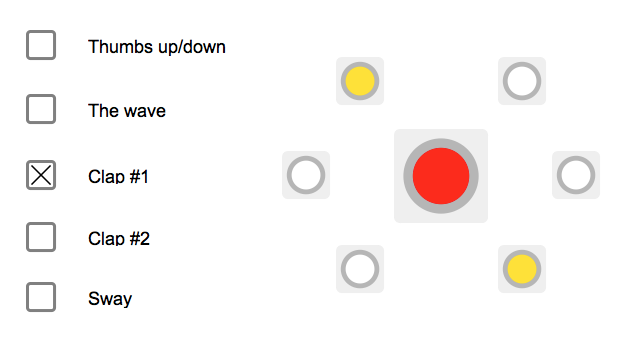
\includegraphics[height=0.2\textwidth]{clap1.png}}
	\hspace{0.1cm}
	\subfloat[Clap-o-meter]{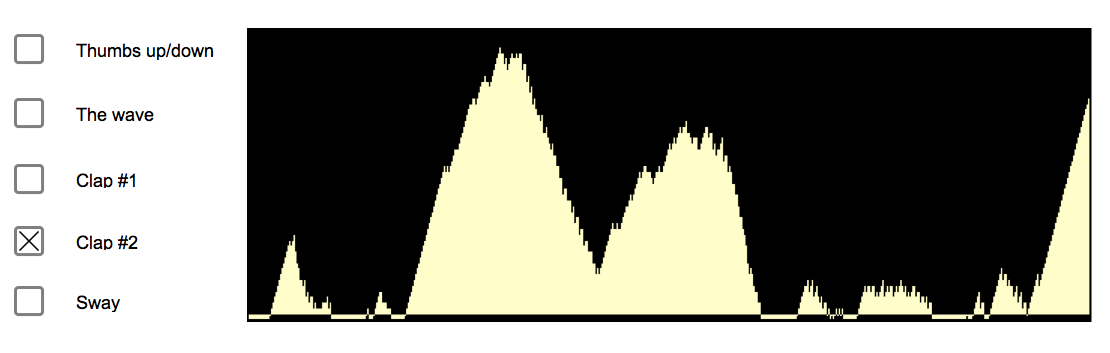
\includegraphics[height=0.2\textwidth]{clap2.png}}
	\hspace{0.1cm}
	\subfloat[Arm swaying]{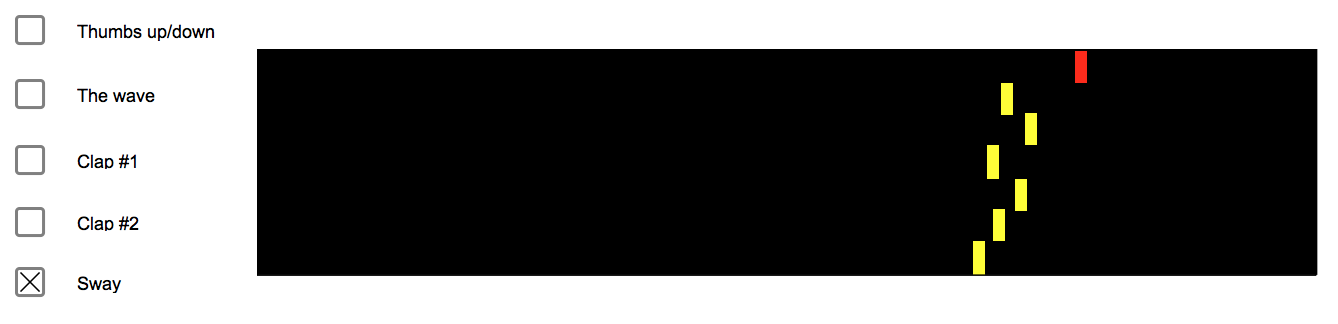
\includegraphics[height=0.2\textwidth]{sway.png}}

	\caption{Input methods}

	\label{prototyping2.2}
\end{figure}
% Put these into a table?
% Use all the final versions of the visualizations?
\fi

Two additional modes were added at this point to act as controls. The first invites users to imitate holding a lighter in the air. This is done by holding the Wii controller upright and pressing the A button, causing LED objects on the screen to illuminate. I included this button-based input to observed how user response compared to that of a motion-based input. In the final mode, users are simply told to dance. The visuals displayed on screen are generated randomly; the users are not actually controlling anything. This was included to see how users responded when the effect of their actions was not clear.

In preparation for the exhibition, I modified the patcher to function as an installation. An auto-play function was implemented; the input methods are looped through automatically, each activated for ten seconds at a time. A short text prompt is displayed to give users a hint at what action they should be performing (``Thumbs up or thumbs down?" ``Sway in sync!" ``Clap-o-meter!" ``Clap in sync!" ``Do the wave!" ``Lighters in the air!" ``Dance!") as shown in Figure \ref{prototyping2.3}. Thus, the system would not require an operator, and users could approach it at any time during the exhibition and test each mechanic.

\begin{figure}[t]
	\centering

	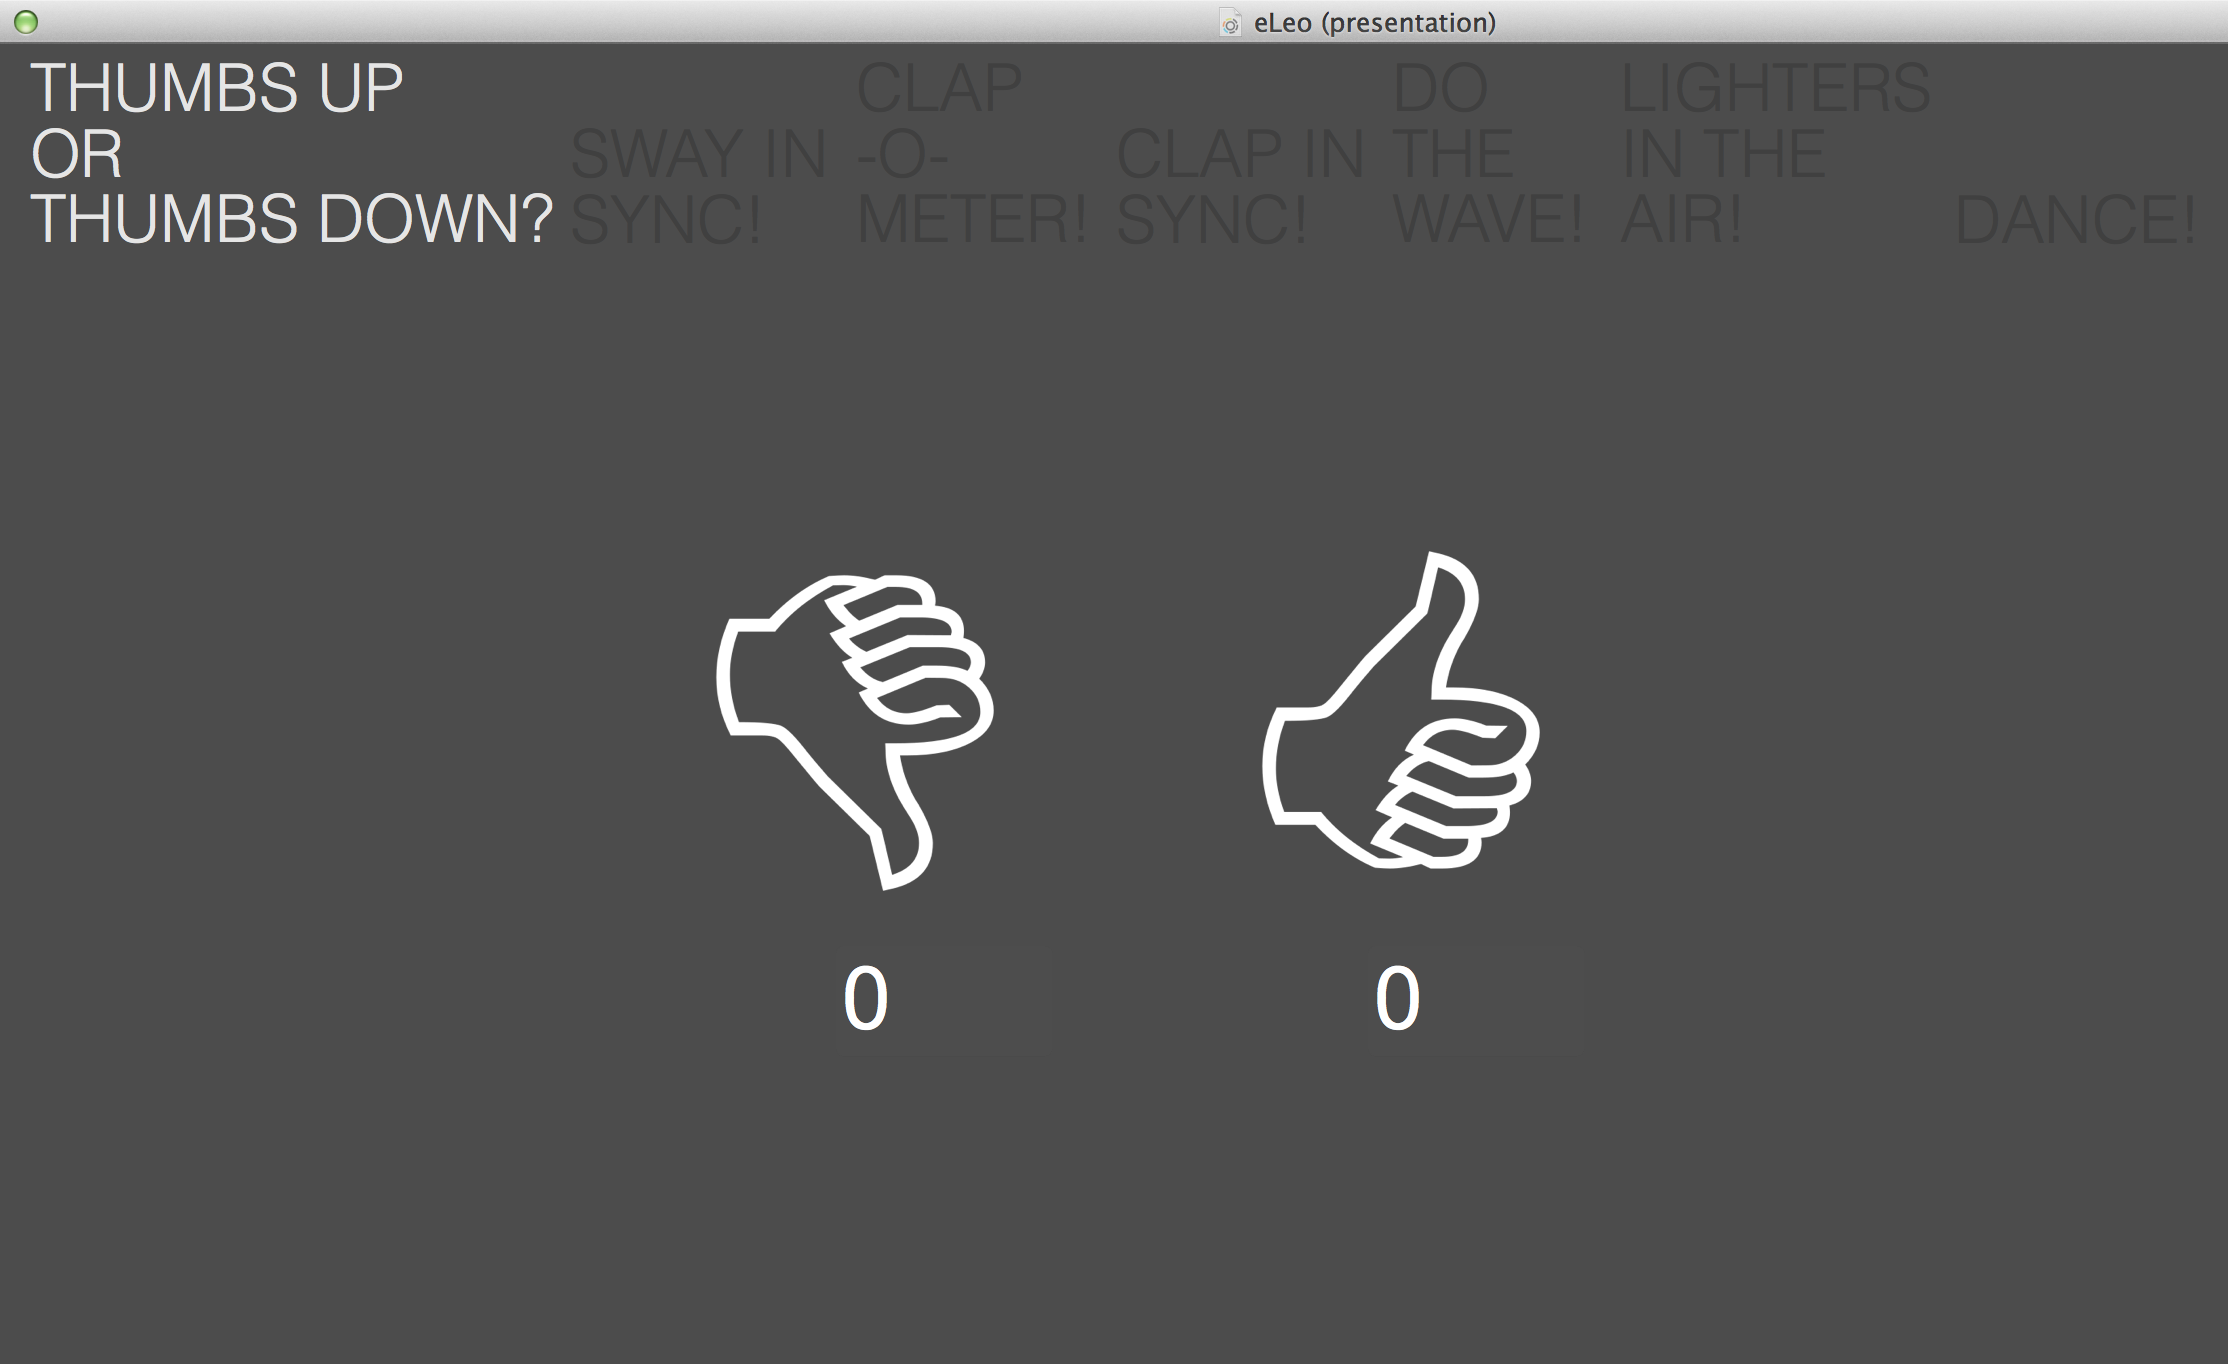
\includegraphics[height=0.4\textwidth]{presentation.png}
	\caption{Input prompts}

	\label{prototyping2.3}
\end{figure}

Lastly, in an effort to make the installation more compelling, part of the VJ system from Prototype \#1 was added to the patcher. Namely, the crossfade system was implemented and connected to each input mechanism. For instance, in swaying mode, if all users swayed their arms to the right, the slider would move to the right and the colour video loop would overtake the black and white loop. In addition to the representative visual feedback already established, then, users could also see how their collective inputs could be used to control a separate system.

\subsection{Testing}
% Explain the details of how participants were recruited, how data was collected, recorded, and processed/analyzed, and the timeline over which this process unfolded

Testing took place during the opening night of the exhibition. The final patcher was projected on a large wall in a darkened room using a short-throw projector. The seven Wii controllers were laid on a table in the middle of the room, their LEDs illuminated, inviting users to pick them up. Figure \ref{prototyping2.4} shows the prototype set up in the exhibition.

\begin{figure}[t]
	\centering

	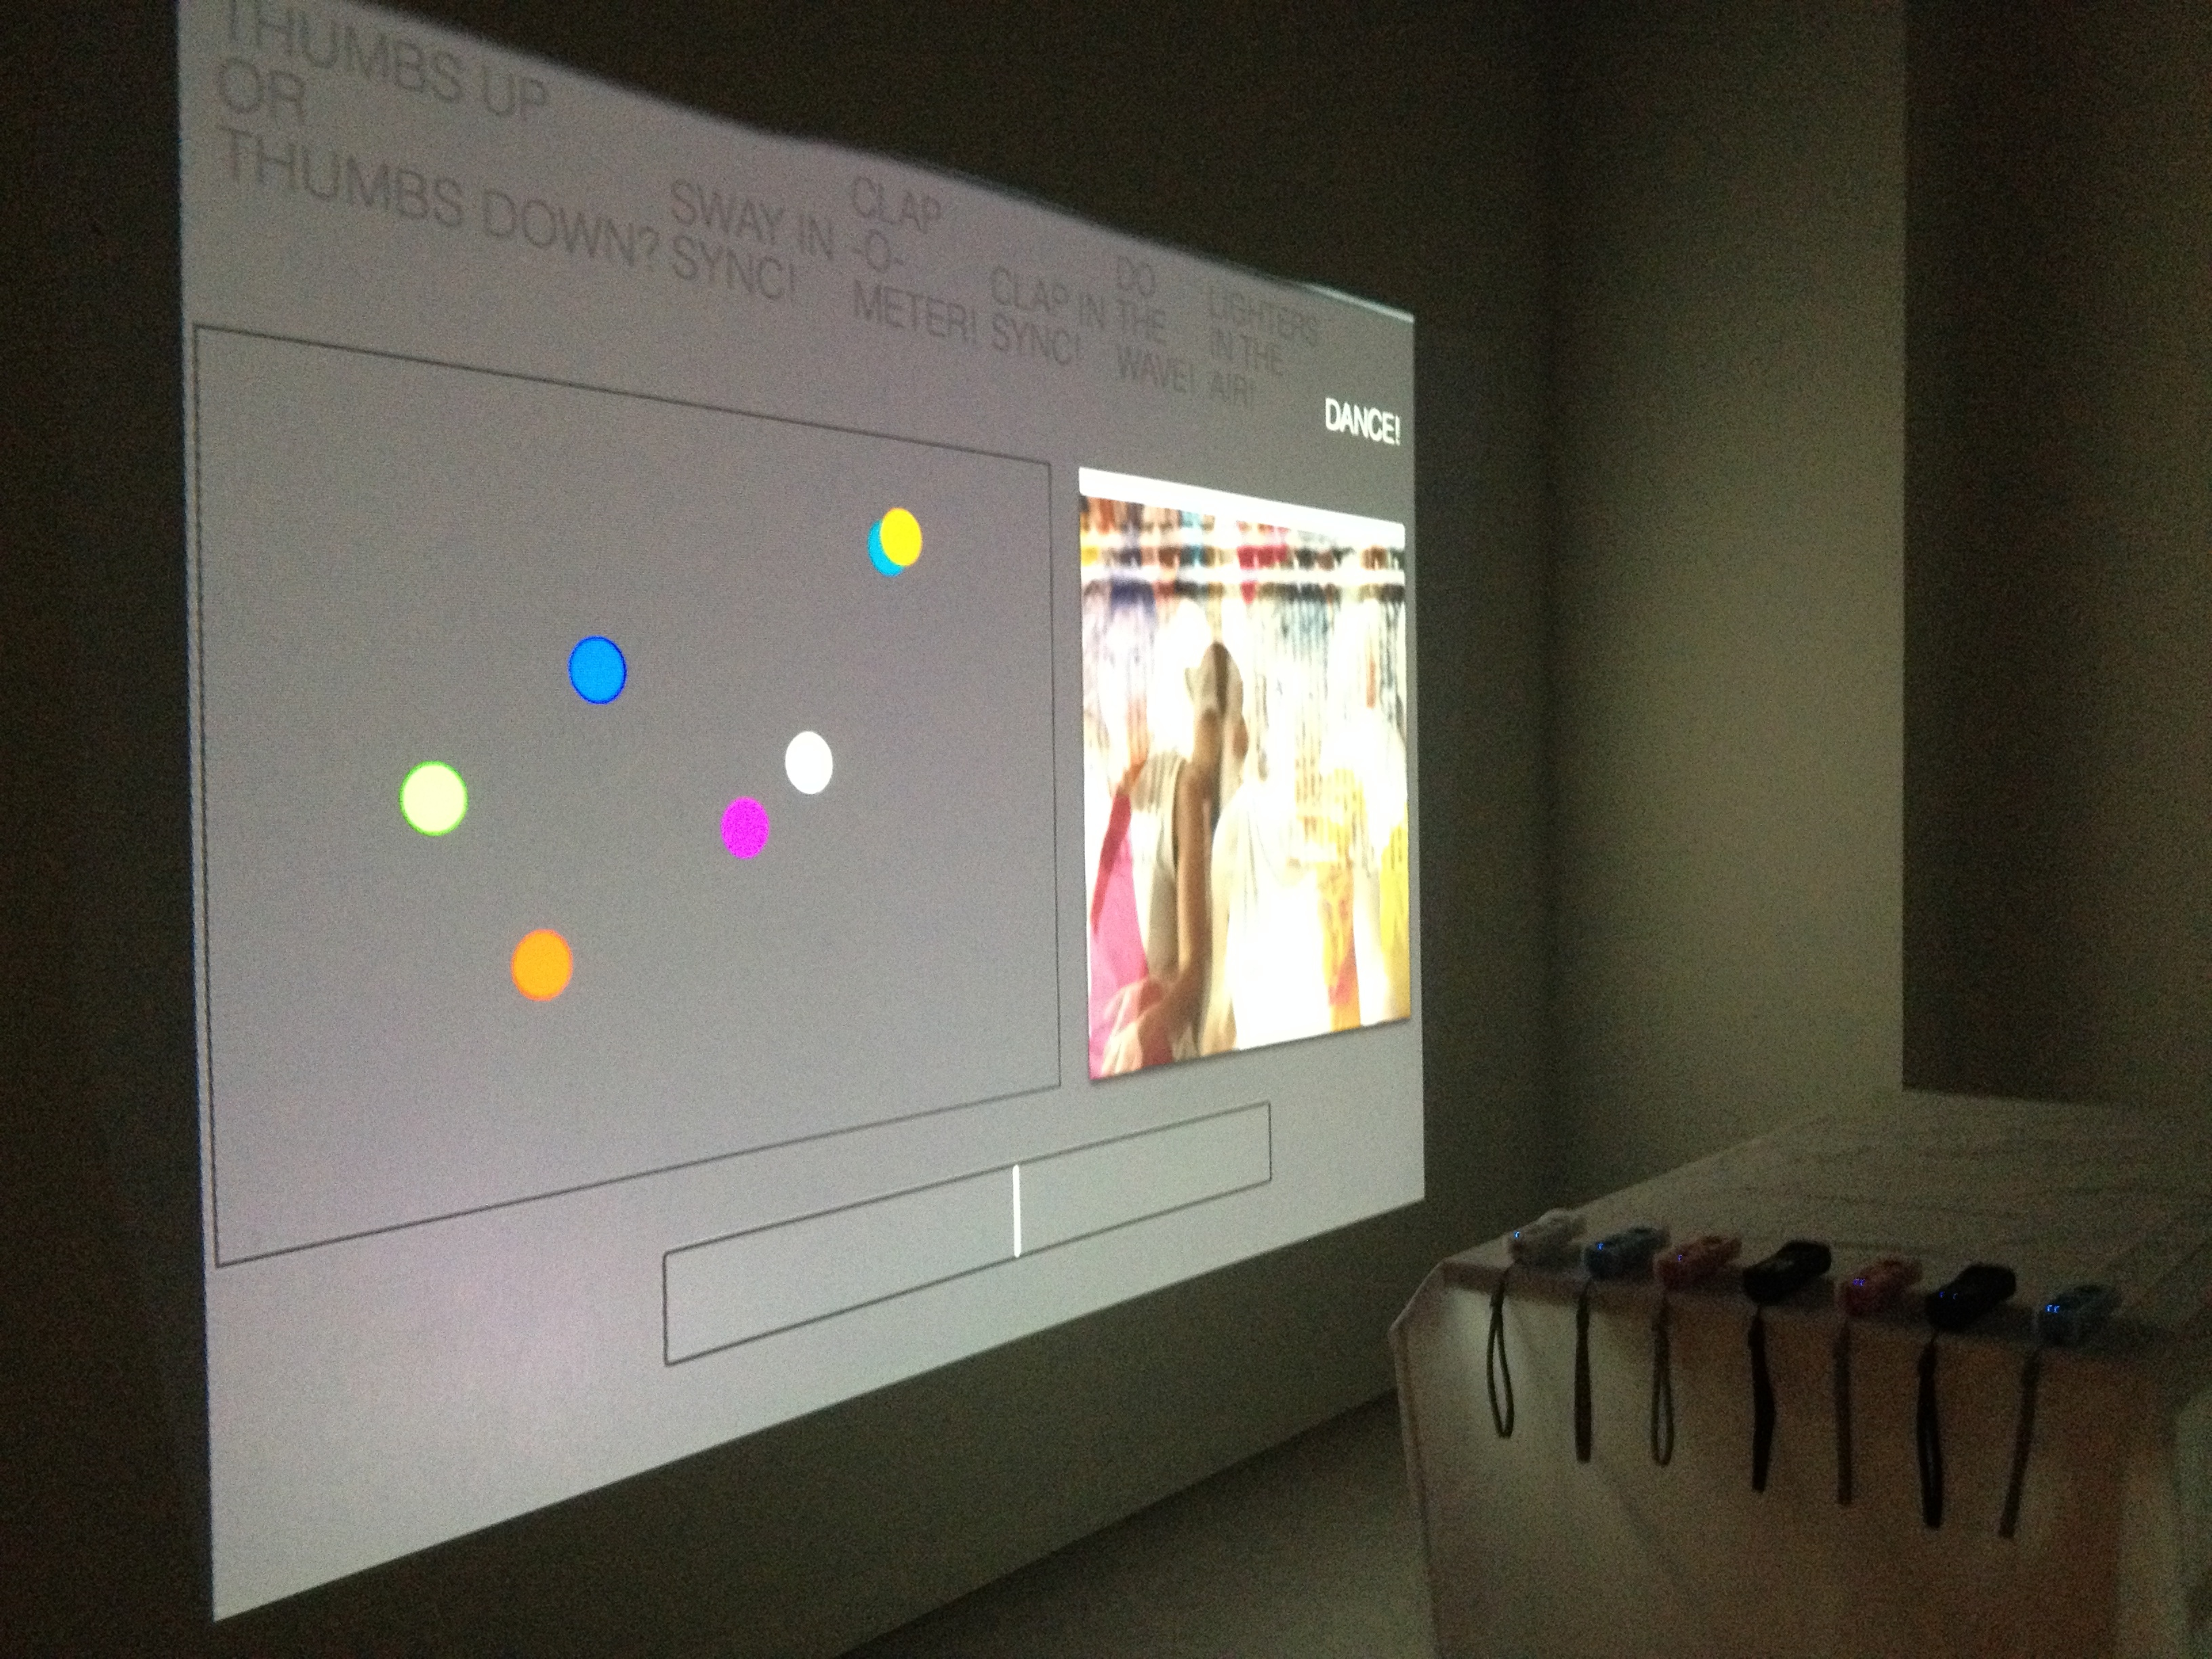
\includegraphics[height=0.4\textwidth]{eleo_1.jpg}
	\caption{Prototype \# 2 installed at the exhibition}

	\label{prototyping2.4}
\end{figure}

Given the casual nature of the event, attendees were relaxed and generally openminded. Groups that entered the room were asked if they were interested in participating in an experiment. Those that accepted were briefed in one of two ways. Half of the groups were told the experiment's motivation -- that I was investigating how audience behaviours could be turned into inputs at live music events. The other half were given no information. I did this to see how users would approach the system if they were given no context. Indeed, some of those who received no information were unsure what was expected of them. Some began pressing buttons on their Wii controller, sometimes holding it up and pointing it at the screen. One user wondered aloud what their goal was.

Those who were given context understood the system much more easily, quickly figuring out that they were to perform physical motions as a group to manipulate the video. Some users invited bystanders to grab a controller and join them, eager to test the system's capabilities. Each input mechanism received different reactions. As I observed and spoke with participants, some general opinions of each method began to surface.

% Thumbs up/down:
Most understood the action quickly, experimenting with combinations. Some tilted the controller left to right, not fully inverting it for thumbs down. The up-versus-down counter seemed random to them at first. Some started shaking the controller. Eventually users coordinated all thumbs up or all thumbs down. Users commented that the thumbs down motion was difficult to perform. Users commented that the up/down action seemed strange to link to the left/right movement of the crossfader slider.

% Sway:
Users had trouble identifying which slider was theirs. Some solved this by shaking the controller violently and observing which slider was moving accordingly. Some users were holding the controller backwards, causing their input to be reversed and adding confusion. Groups eventually coordinated themselves and began swaying in sync. Most users did not raise their arms in the air, instead casually hold the controller in front of them. In conversation, they indicated that they did not feel compelled to since the visuals were already responding. 

% Clap-o-meter:
Since the visualization reacted gradually, users were initially confused. They commented on the slow response. While some said that the visualization was appealing, many agreed that they would preferring seeing individual  Groups eventually worked together to fill up the clap-o-meter. Users were unsure how to clap with the controller in their hand; some complained that it was painful to hit it against their palm. Users tired of this mode quickly.

% Clap in sync:
In most groups, one user would lead the others by counting out a time. Users commented that it was a fun challenge to try to clap in sync. However, once syncopation was achieved, most groups felt they had achieved what was expected and stopped. Some commented that the minor lag in the visualization was distracting.

% The wave:
Nearly all users instantly understood the prompt and were eager to raise their arms in the air. Figure \ref{prototyping2.5} shows three participants performing the wave input. One group did not communicate and instead just watched their own slider, but most cooperated to raise their arms simultaneously. One group organized themselves in a row such that they were in the same order as their sliders on screen. Users enjoyed the appearance of this visualization. Although, a particularly thought-provoking comment was made by one user: this visual representation of the wave was less appealing than the wave itself. 

\begin{figure}[t]
	\centering

	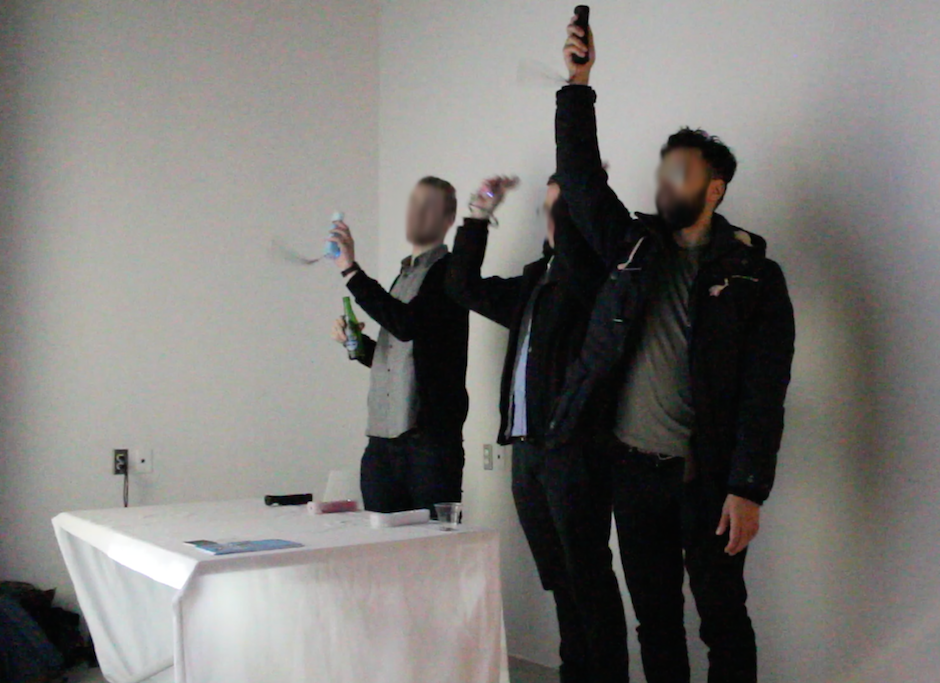
\includegraphics[height=0.4\textwidth]{testing.png}
	\caption{Three users experiment with the prototype}

	\label{prototyping2.5}
\end{figure}

% Lighters:
Most users instantly understood this as well. Some tried to see if pushing the button rapidly would create a different response. Some groups worked together to light up all the LED objects together. This seemed unexciting to users; one vocalized her boredom.

% Dance:
Most users responded to the prompt without hesitation and began moving. Others were clearly not comfortable doing so. Many stared at the random visualizations and tried to make sense of their role. Some were annoyed when told their input had no effect.

In multiple modes, users noted that they were not paying attention to the video and were rather focusing their attention on the sliders or LED objects. One user suggested that if the system were incorporated into a live performance, the video clips could be two different live feeds of the performance itself.

\subsection{Analysis}

% The buttons were misleading

% Individual visualizations for each user (i.e. not Thumbs up/down or Clap-o-meter)

% On/off is most appealing. Choosing between two options caused confusion (i.e. no more left/right voting). This is just like regular audience behavior I guess?

% Collaboration came naturally and was enjoyable

% Direct control of visual elements trumps indirect control (i.e. ditch the video crossfading)

% Users should be able to opt out without affecting others' experiences (i.e. not Thumbs up/down or Clap-o-meter)

% No forced goals (i.e. no prompts to perform in sync). Allow for creativity.

% Be clear about the rules of the system or users will begin experimenting and become distracted

% The output must be more captivating than the input (i.e. no digital wave)


\section{Prototype \#3}

This chapter covers the development of the third and final prototype. I explain the design goals, the creation process, and the user testing that was carried out. The chapter closes with a discussion on the significance of the prototype.

\subsection{Motivation}

The final prototype took the form of a collaboration with one of the ethnography subjects, local musician Christian Hansen. After our interview, he expressed interest in incorporating one of my prototypes into a performance. My ethnographic study made it clear that each performer has a unique opinion on what makes a great performance; thus, I knew that it would be important to develop a new prototype with Christian and ensure that the system reflected his performance style.

The current incarnation of the Christian Hansen band features Christian providing lead vocals and Molly playing keyboard, performing backup vocals, and controlling backing tracks. Both bring high energies to their performances; Christian frequently moves around the stage, dances, and sings very expressively, and Molly, despite being stationed behind a keyboard stand, continuously moves to the music as well. The band does not typically use any more equipment than is needed. They aim to make a big impact through simplicity and rawness. As explained in Chapter 5, Christian will often involve the audience, encouraging singalongs and moving between the stage and the crowd. He feels that it is his job to maximize the audience's energy level.

The band expressed interest in allowing the audience to control their light show in some way. Christian wanted a system that could unite audience members without turning into a distraction from the music. He also expressed concern about giving the audience too much control; only the band should be able to dictate the flow of the performance. Christian hoped that the technology would create a controlled environment that left some room for some spontaneity and uncertainty. My goal, then, was to develop a system that satisfied these wishes. However, it was important for design decisions to also be based in the knowledge gained from previous prototypes.

I decided to give each audience member control over one light in an array of lights to be located on stage. An audience members would receive a simple wireless device to control their light, which would provide obvious and consistent visual feedback. Users would only be faced with two options -- turn the light on momentarily or leave it off. As the last prototype revealed, limiting the audience's options in this way would reduce the opportunities for confusion; this feature also reflects the artist's desire for simplicity. This one-light/one-person mechanic had additional benefits. If a user decided not to participate, for instance, it would not have a direct effect on the other users' experiences. The system is not inherently goal oriented, so a user is free to experiment without concern for what the others are doing. That being said, there could be benefits to collaboration; for example, if the crowd worked together to turn on all of the lights in sync, the outcome would likely be more rewarding than if everyone acted independently. Organizing synchronized inputs proved to be enjoyable for participants in the previous experiment. Lastly, it was decided that lights would be activated by clapping with the device. Out of the methods tested for the last prototype, I felt that this made the most sense for the system; however, some adjustments would be needed to address the criticisms that were received. Namely, the action had to be made more comfortable to perform, and the lights' response time had to be minimized.

After presenting the initial concept to the band, some further adjustments were made. It was decided that hanging the lights from the keyboard would allow for the easiest setup and provide sufficient visibility to the crowd. Next, Christian and Molly expressed interest in being able to interact with the lights themselves. We agreed that it would be intriguing to design the lights such that the performers could pick them up; this could lead to unusual new interactions between audience and performer. Another point of discussion was how long the audience would be controlling the lights. The band and I both felt that the system should not be active for the whole performance, speculating that the audience would grow tired of it. We agreed to introduce the devices for the last two songs of the show. This would give the crowd sufficient time to warm up to the band and serve as a surprising finale. Rather than leaving the lights inactive, however, it was decided to incorporate them in a programmed light show until the audience was given control.

Figure X shows a diagram illustrating the system's functionality.

% Figure X

% User testing would help identify...

\subsection{Development}

%Implemented Maxduino to control Arduino using Max. Can control LEDs via Max. Added Wii controller control. Can now use multiple Wii controllers to turn on multiple LEDs via Arduino via Max. LED and rumble feedback implemented in Wii controllers. Figure \ref{prototyping3.1}.
The final prototype was built off of the reliable system used in the previous experiments. Audience members would be given Wii controllers, and OSCulator and Max would process the data they generate. In order to operate lights, however, I also needed to make use of an Arduino microcontroller. This compact and versatile board could be easily programmed to operate an array of lights. After installing a library called Maxuino\footnote{\url{http://www.maxuino.org}}, I was able to easily send instructions to the Arduino from the Max environment. As an initial test, I pulled button-press data from on Wii controller and connected the Arduino to an LED; I was successfully able to illuminate the LED by pressing the controller's A button, as shown in Figure \ref{prototyping3.1}.

\begin{figure}[t]
	\centering

	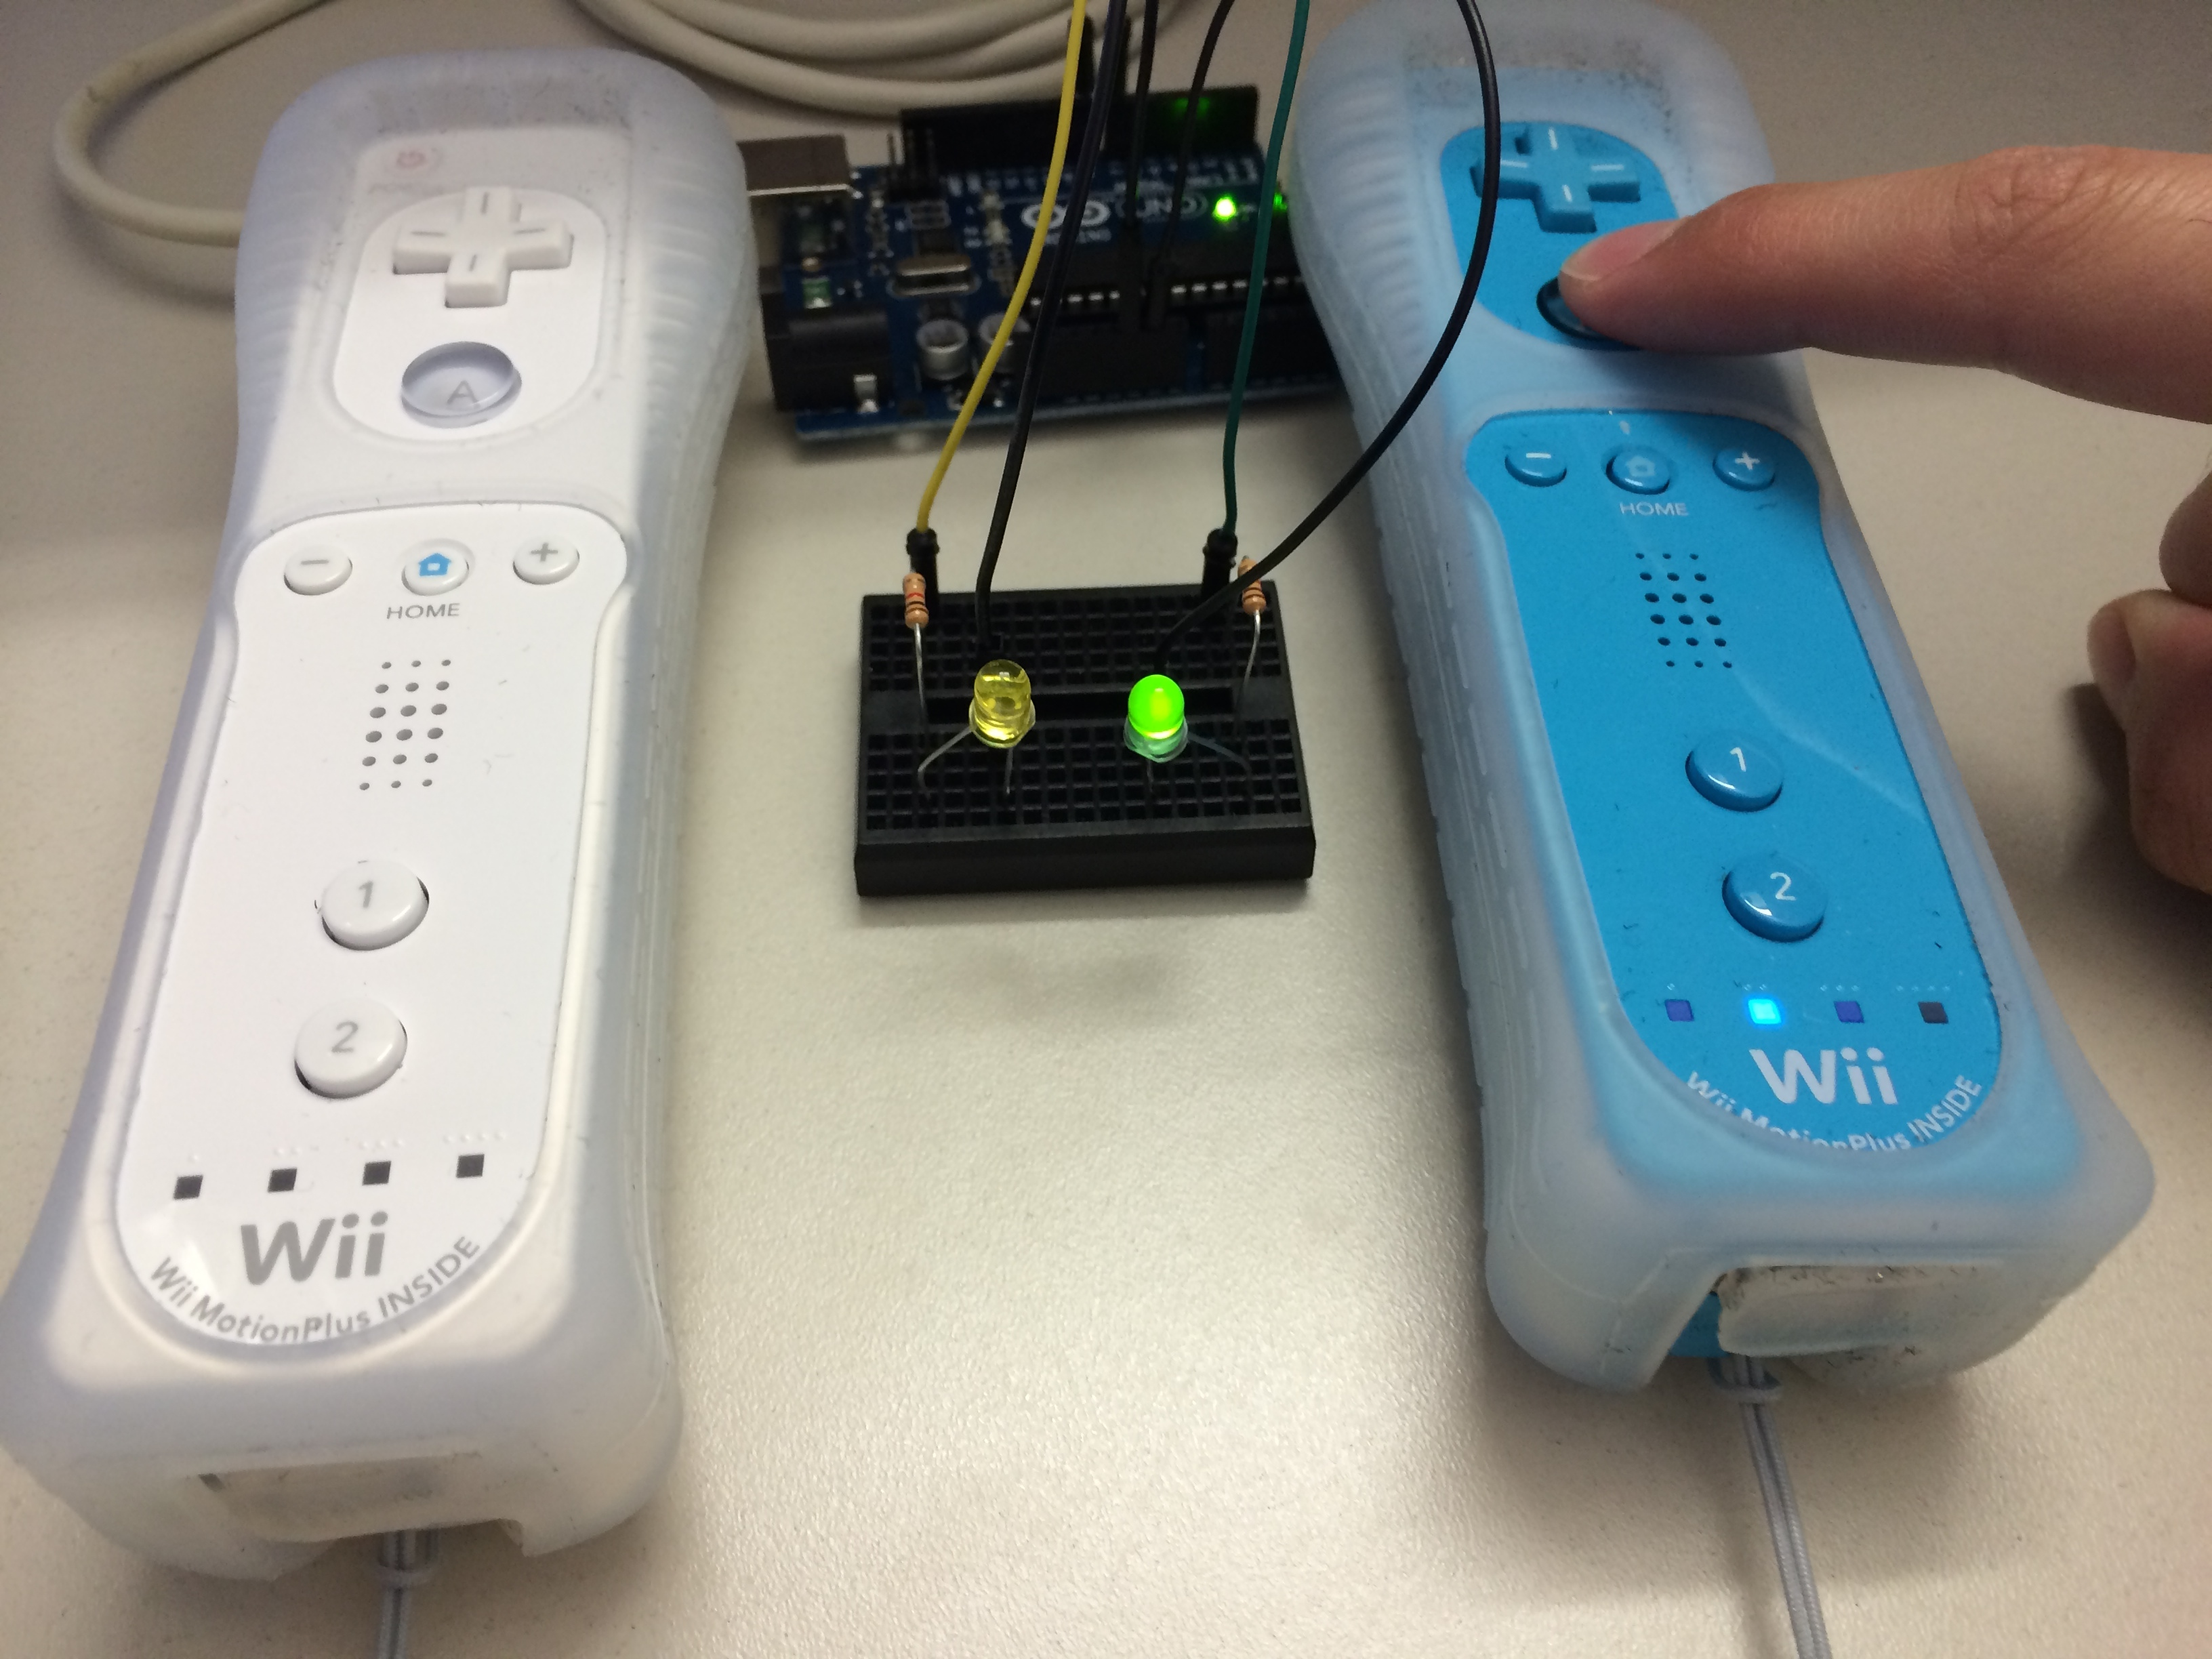
\includegraphics[height=0.4\textwidth]{wii_led.jpg}
	\caption{Turning on an LED with a Wii controller using Maxuino}

	\label{prototyping3.1}
\end{figure}

Tested incandescent bulbs; drew too much current and took too long to turn on. Tested bright LED lamp -- requires 12 V, ~100 mA each. Figure \ref{prototyping3.2}.

\begin{figure}[t]
	\centering

	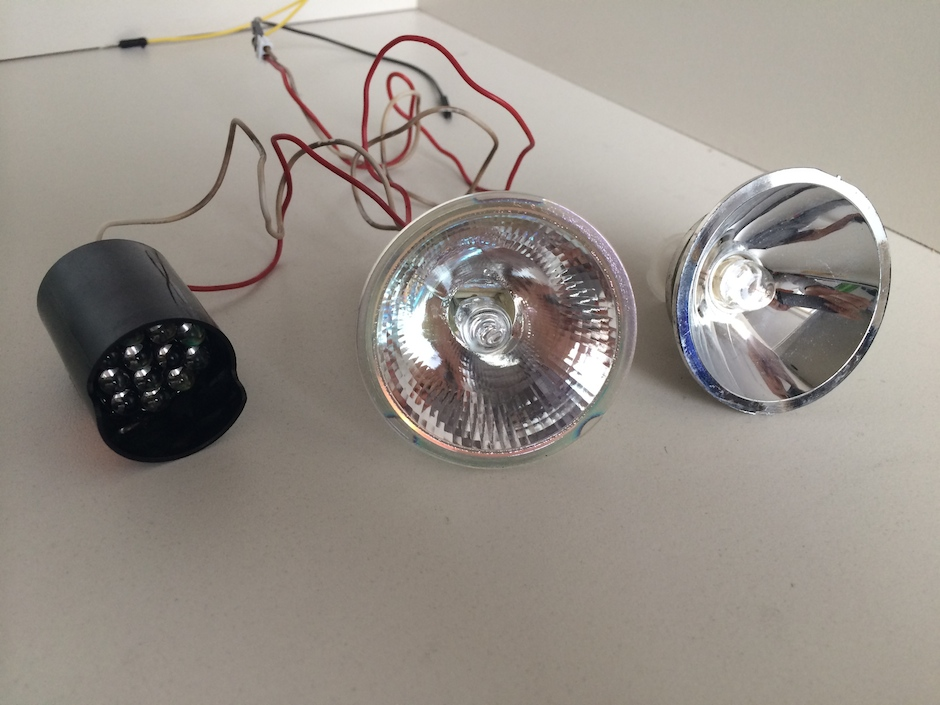
\includegraphics[height=0.4\textwidth]{light_1.jpg}
	\caption{Testing different types of lights}

	\label{prototyping3.2}
\end{figure}

Made working relay circuit with LED lamps -- Arduino switches TIP120s and turns lamps on and off. Made circuit with two relays and two LED arrays. Created Arduino sketch to alternate the arrays on and off. Acquired 12 V / 1 A power source and incorporated it into the circuit. Figure \ref{prototyping3.3}.

\begin{figure}[t]
	\centering

	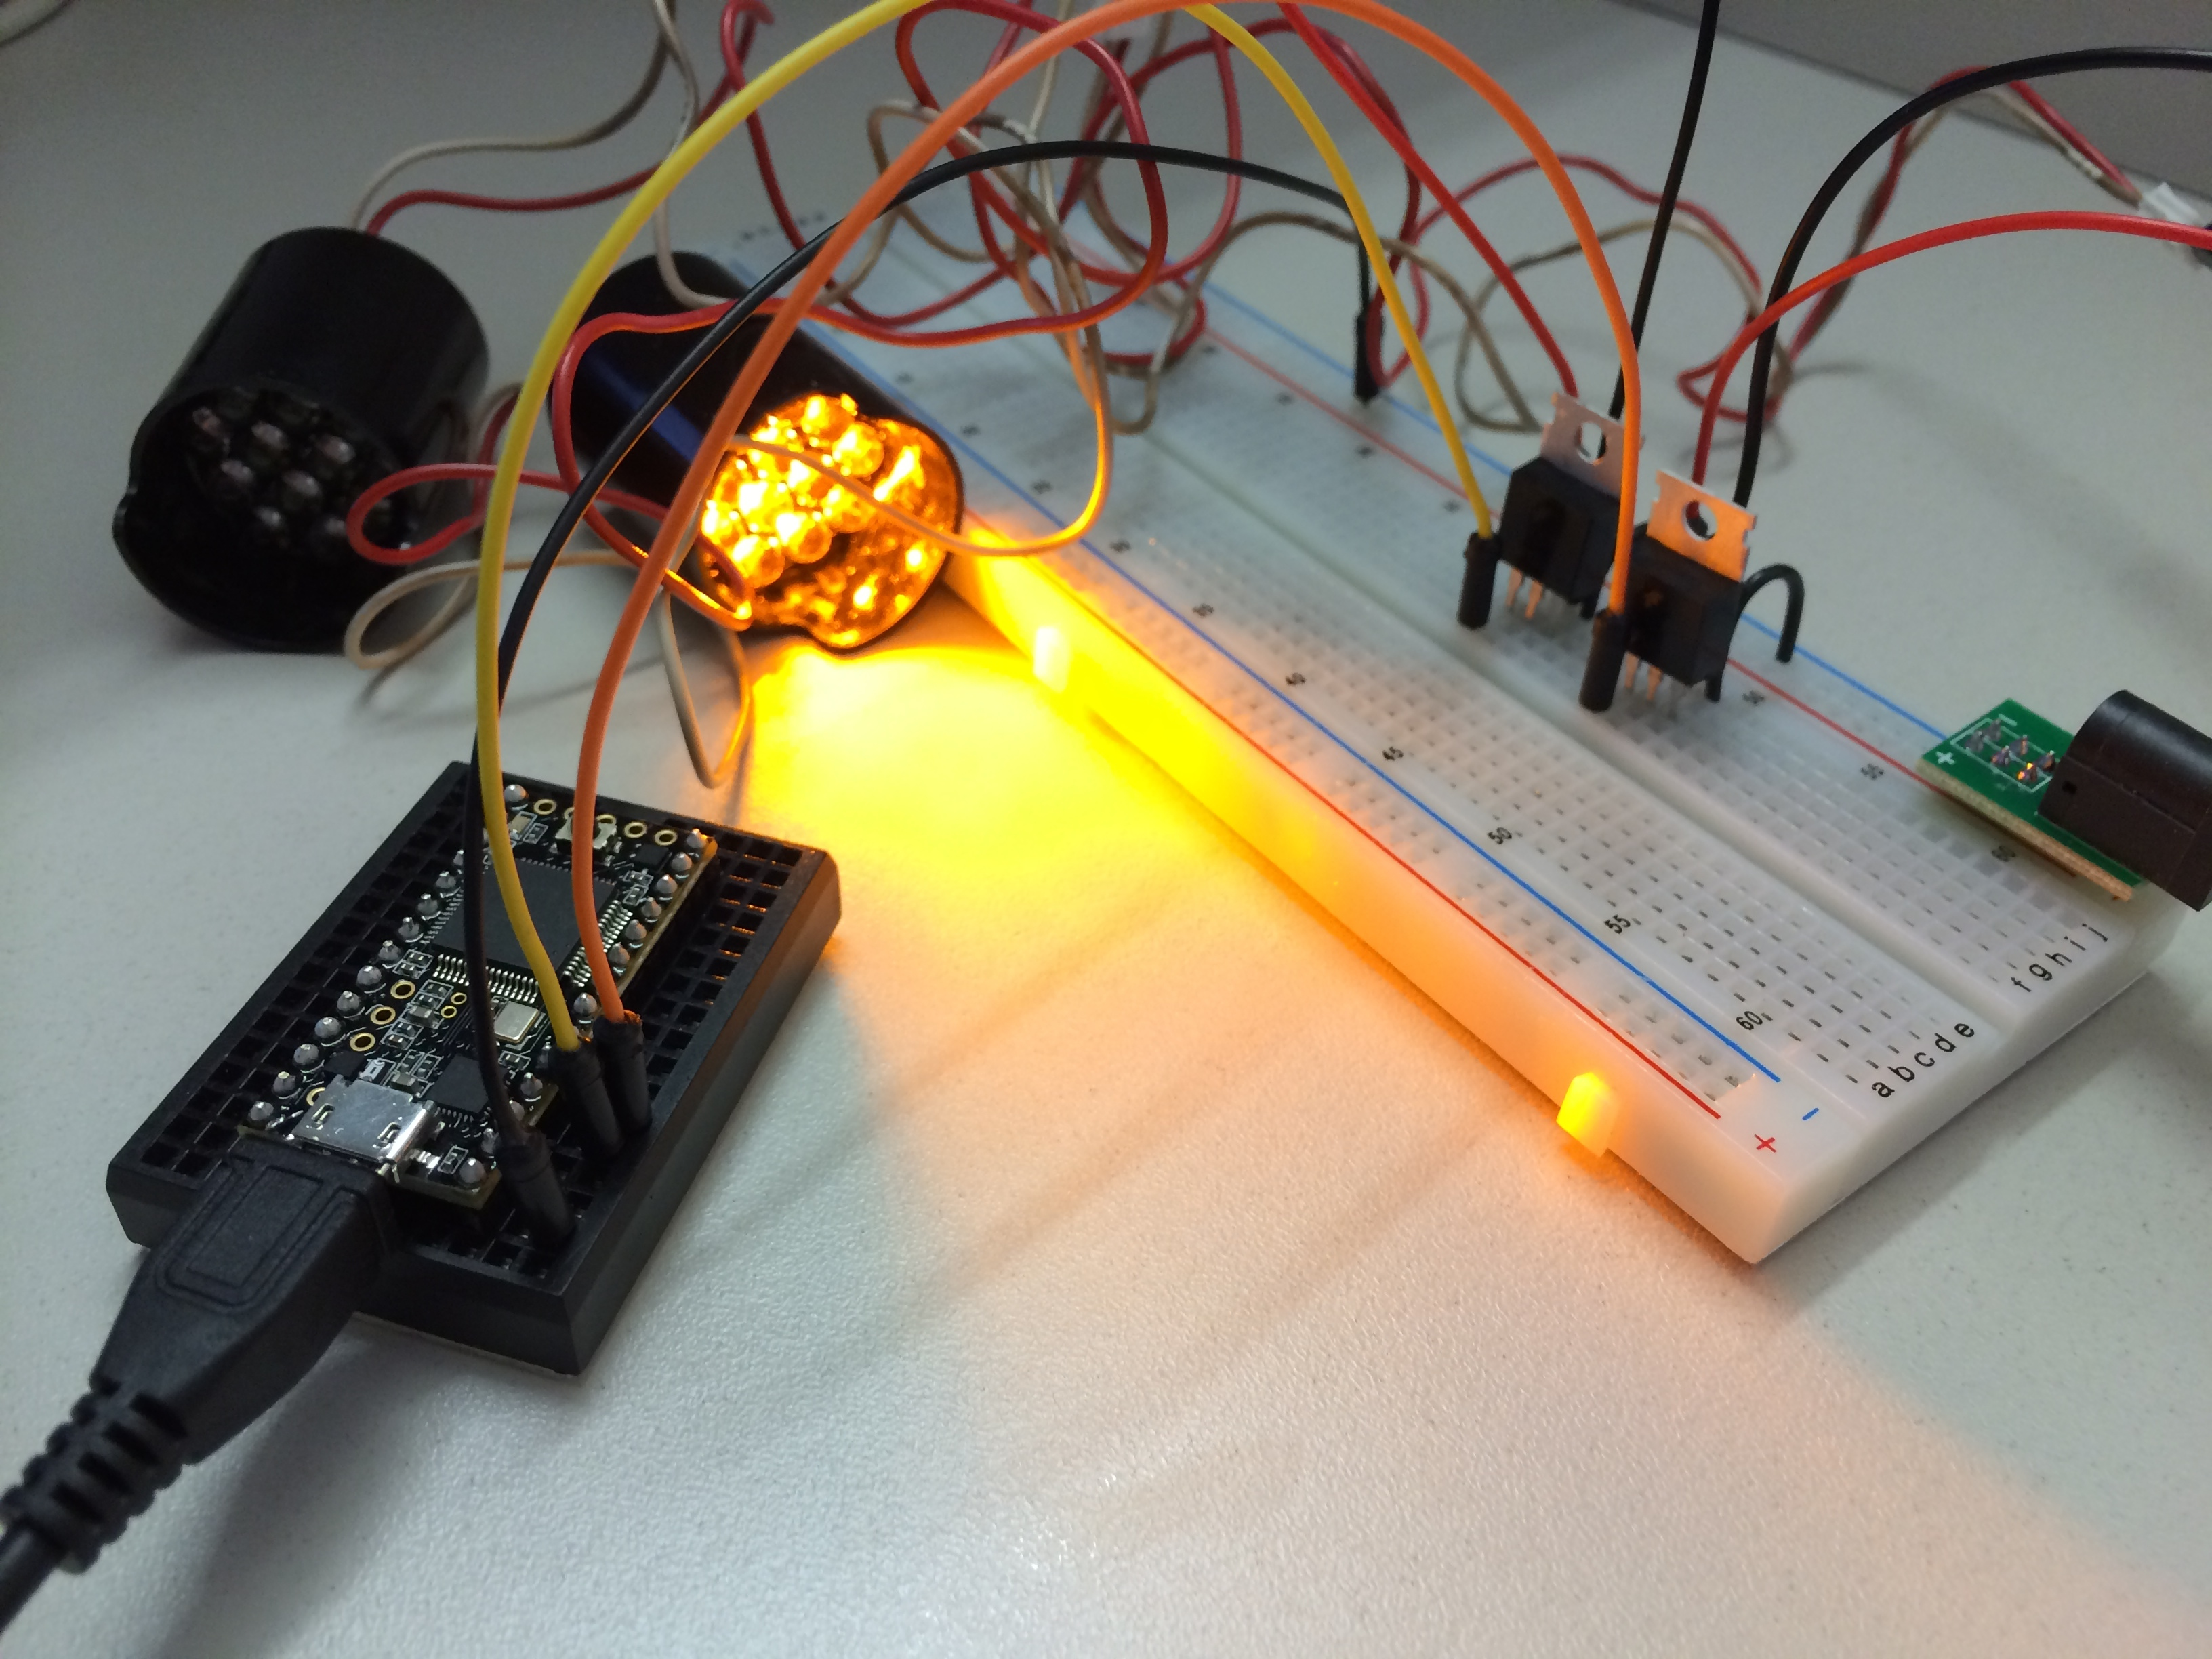
\includegraphics[height=0.4\textwidth]{light_2.jpg}
	\caption{Operating two lamps using transistors and an Arduino}

	\label{prototyping3.3}
\end{figure}

Made clap-operated lighting system using 3 Wii controllers and 3 LED arrays. Networked two MacBooks together through OSCulator to allow for up to 14 Wii controllers. Set up OSCulator routing; 6 Wii controllers on second MacBook send data to first MacBook over LAN; all connections both ways work as expected.

Replaced TIP120s with P2N2222A transistor -- smaller, more available, still handles the current. Soldered LED control board. Installed in project box. Figure \ref{prototyping3.4}

\begin{figure}[t]
	\centering

	\subfloat[LED control board]{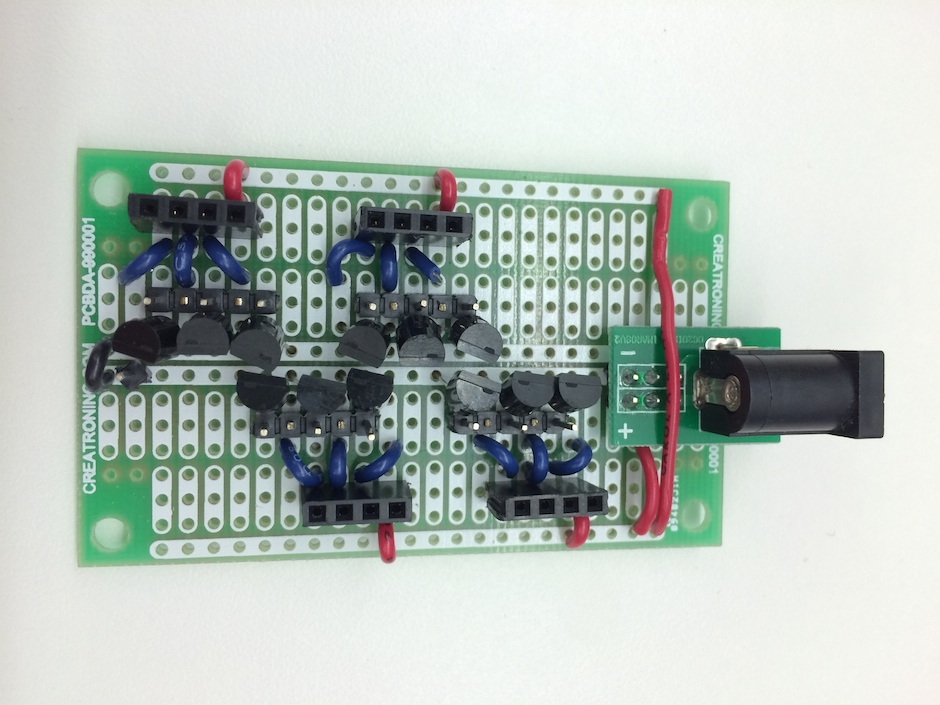
\includegraphics[height=0.36\textwidth]{board.jpg}}
	\hspace{0.1cm}
	\subfloat[Board connected to Arduino Uno]{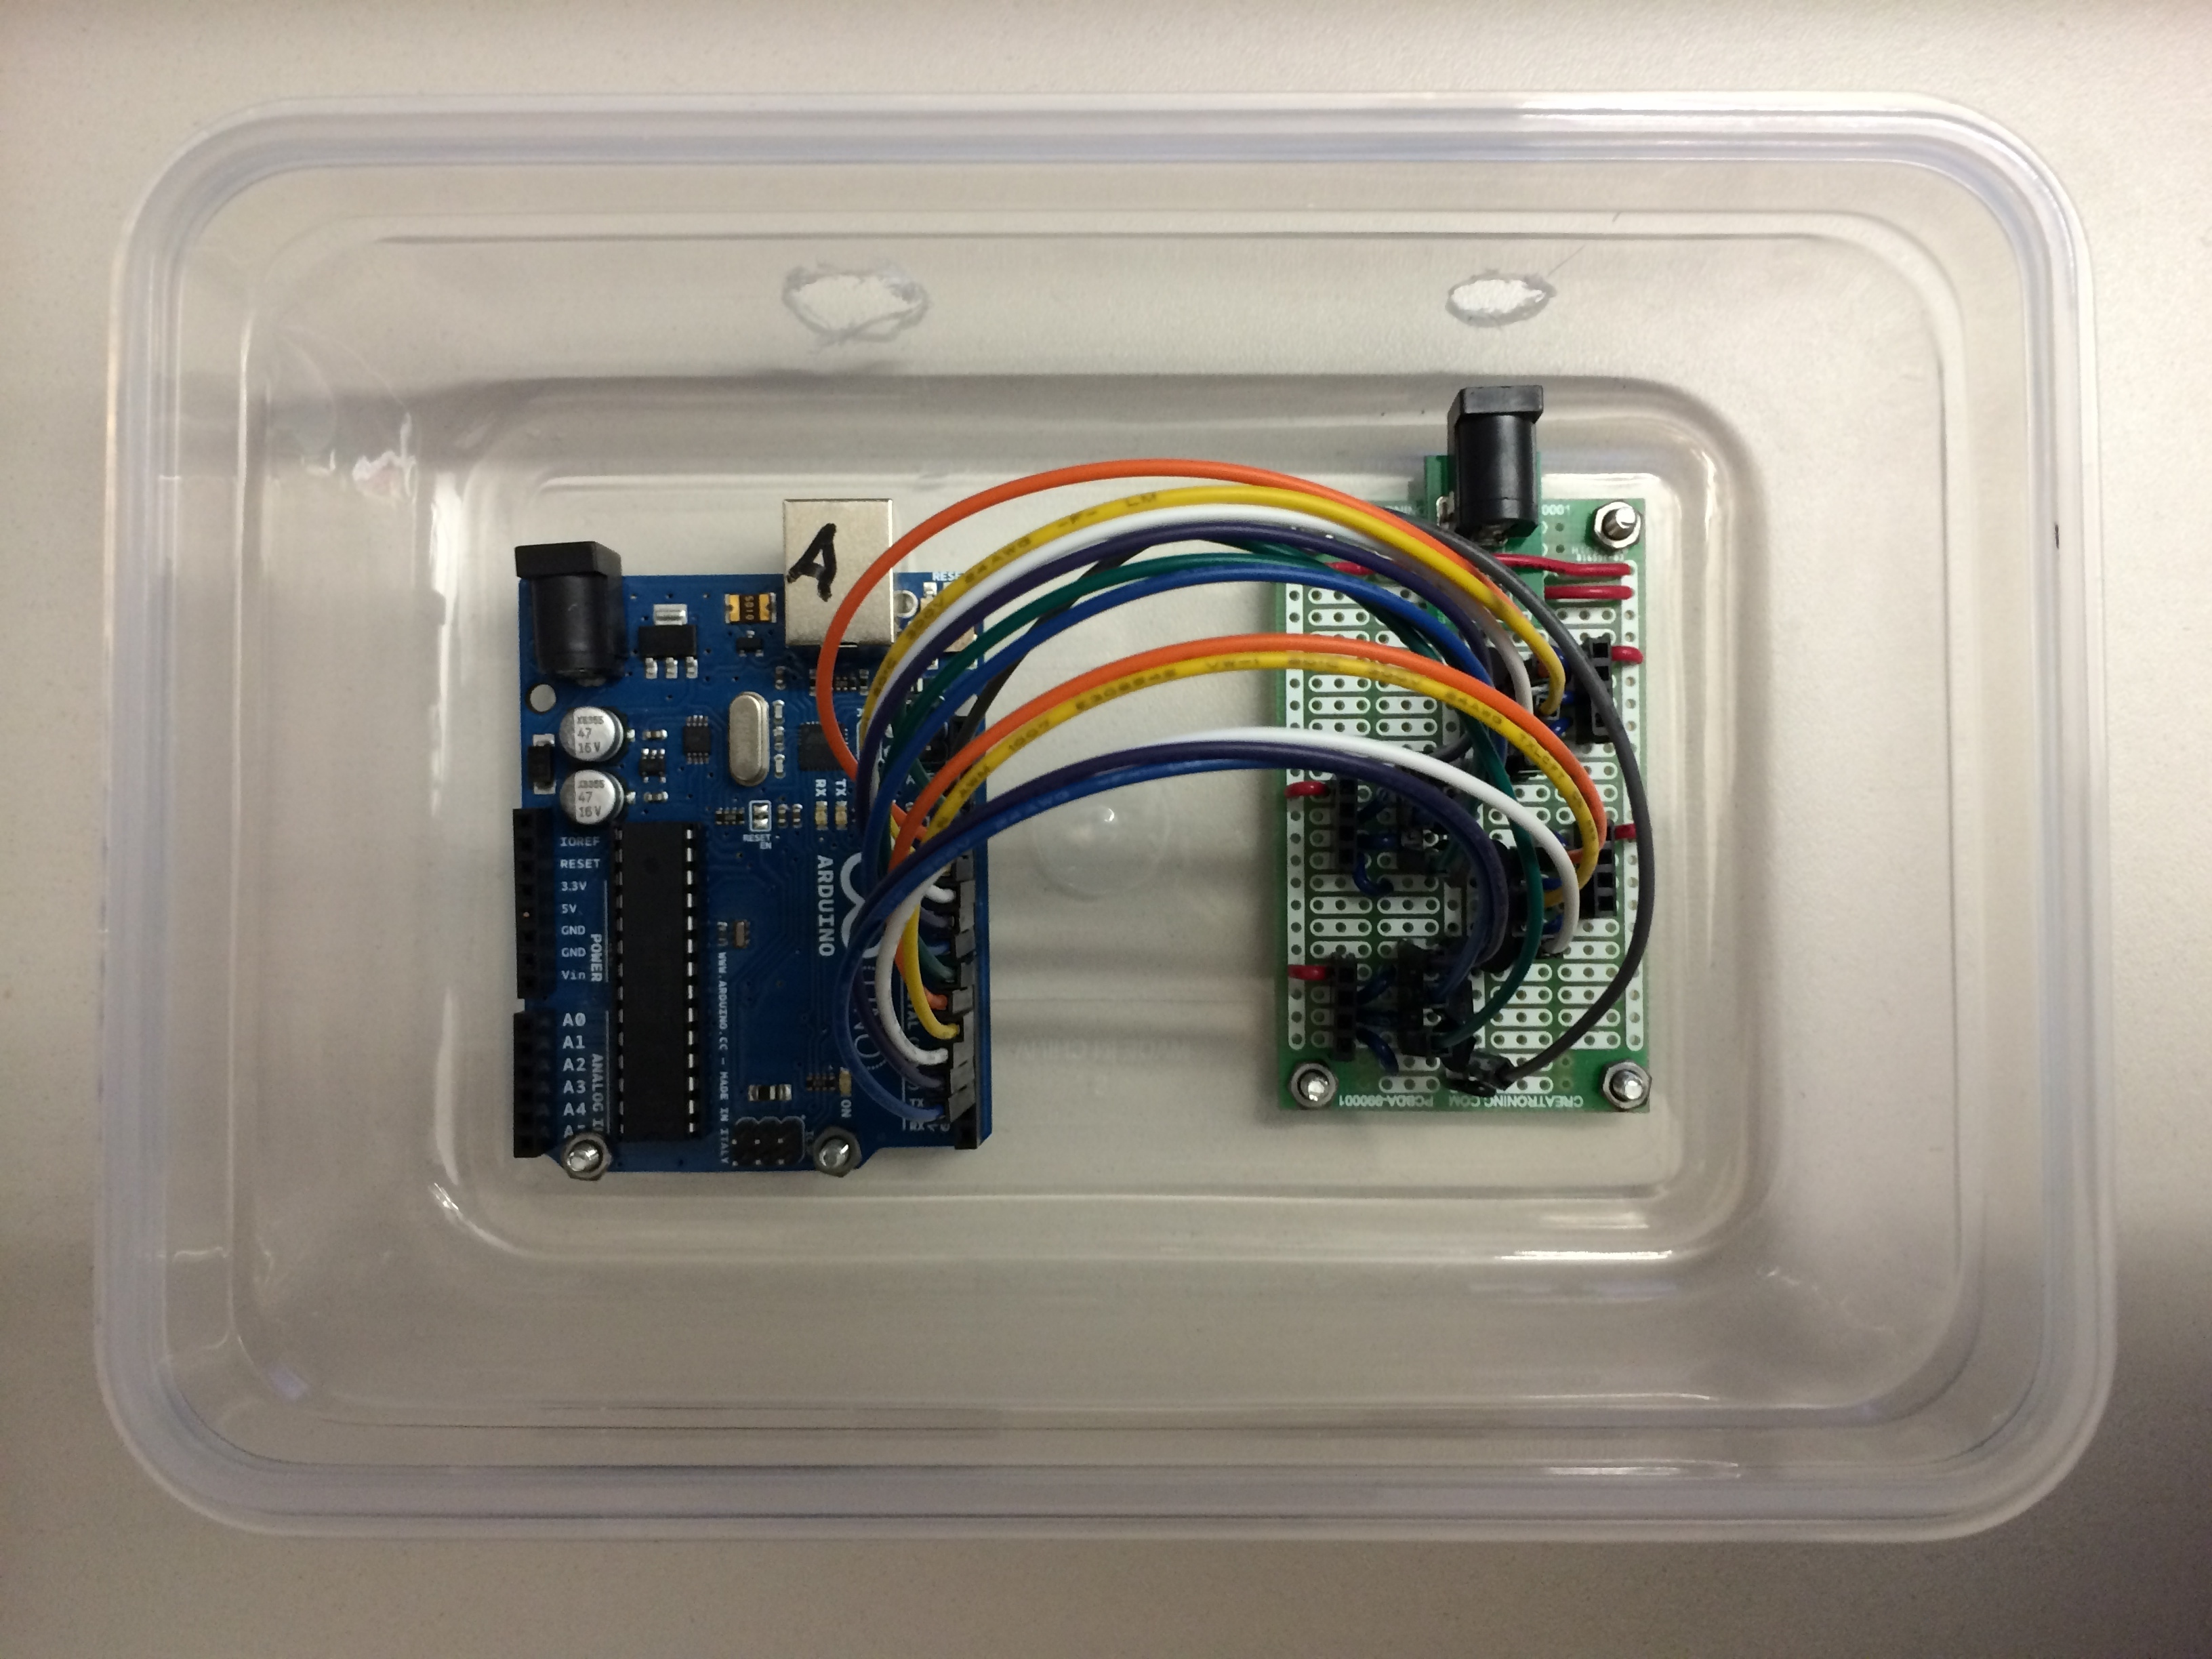
\includegraphics[height=0.36\textwidth]{electronics.jpg}}

	\caption{Prototype \#3 electronics}

	\label{prototyping3.4}
\end{figure}

Laser cut acrylic to make first prototype of light stand. Tested it with LED lamps. Laser cut second version of light stand x 4. Installed lamps and wire. Figure \ref{prototyping3.5}.

\begin{figure}[t]
	\centering

	\subfloat[Laser-cut acrylic]{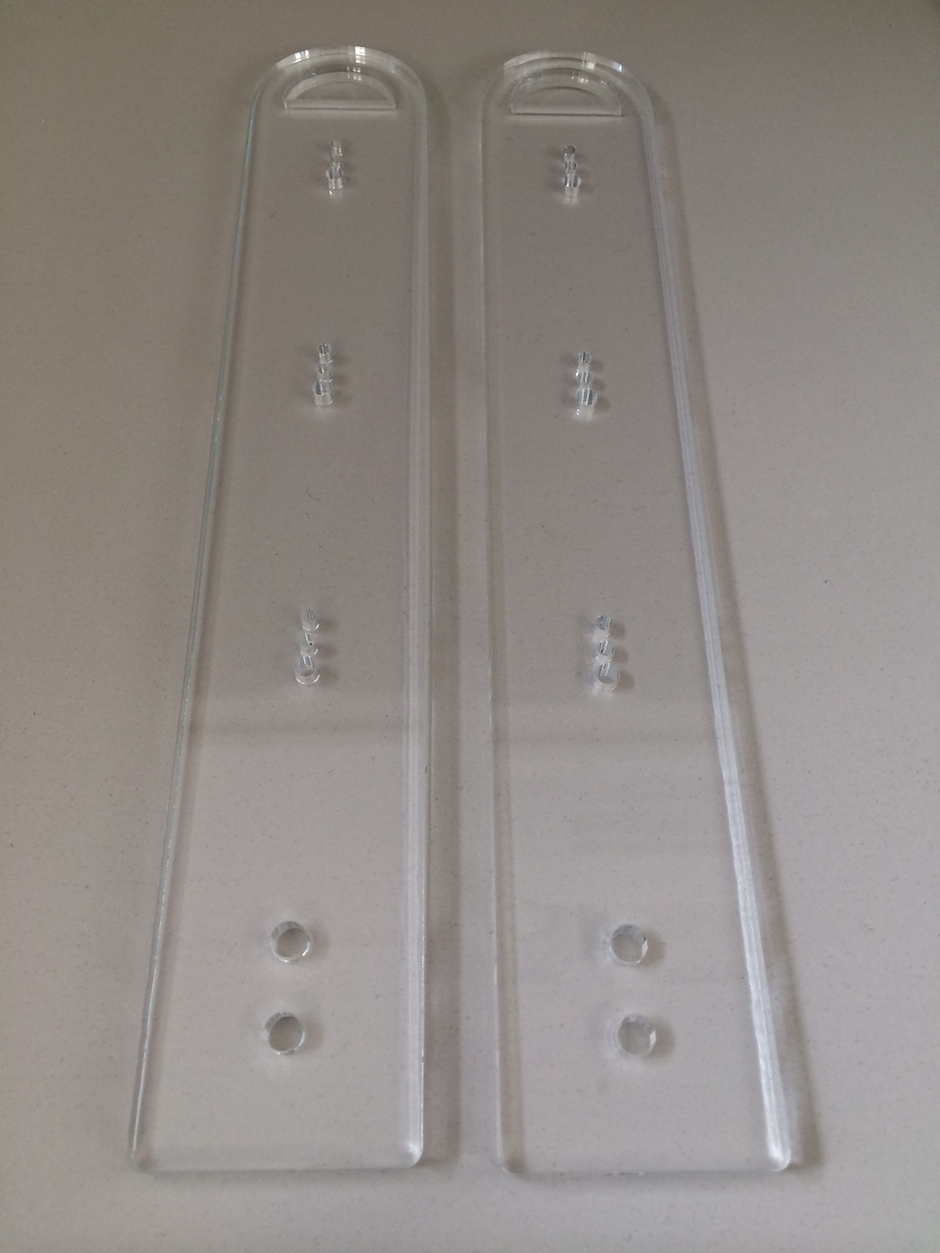
\includegraphics[height=0.4\textwidth]{rigs_1.jpg}}
	\hspace{0.1cm}
	\subfloat[Lamps and wire installed]{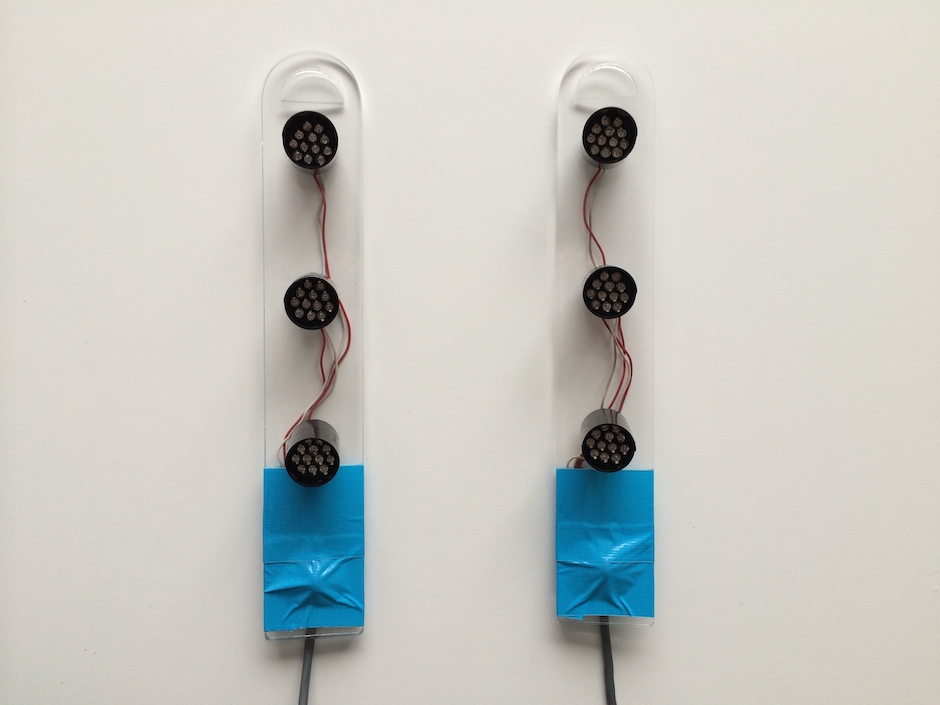
\includegraphics[height=0.4\textwidth]{rigs_2.jpg}}

	\caption{Light stands}

	\label{prototyping3.5}
\end{figure}

Incorporated enable/disable system for each lamp. Created light show programming system. Created a monitoring system in Max. Figure \ref{prototyping3.6}.

\begin{figure}[t]
	\centering

	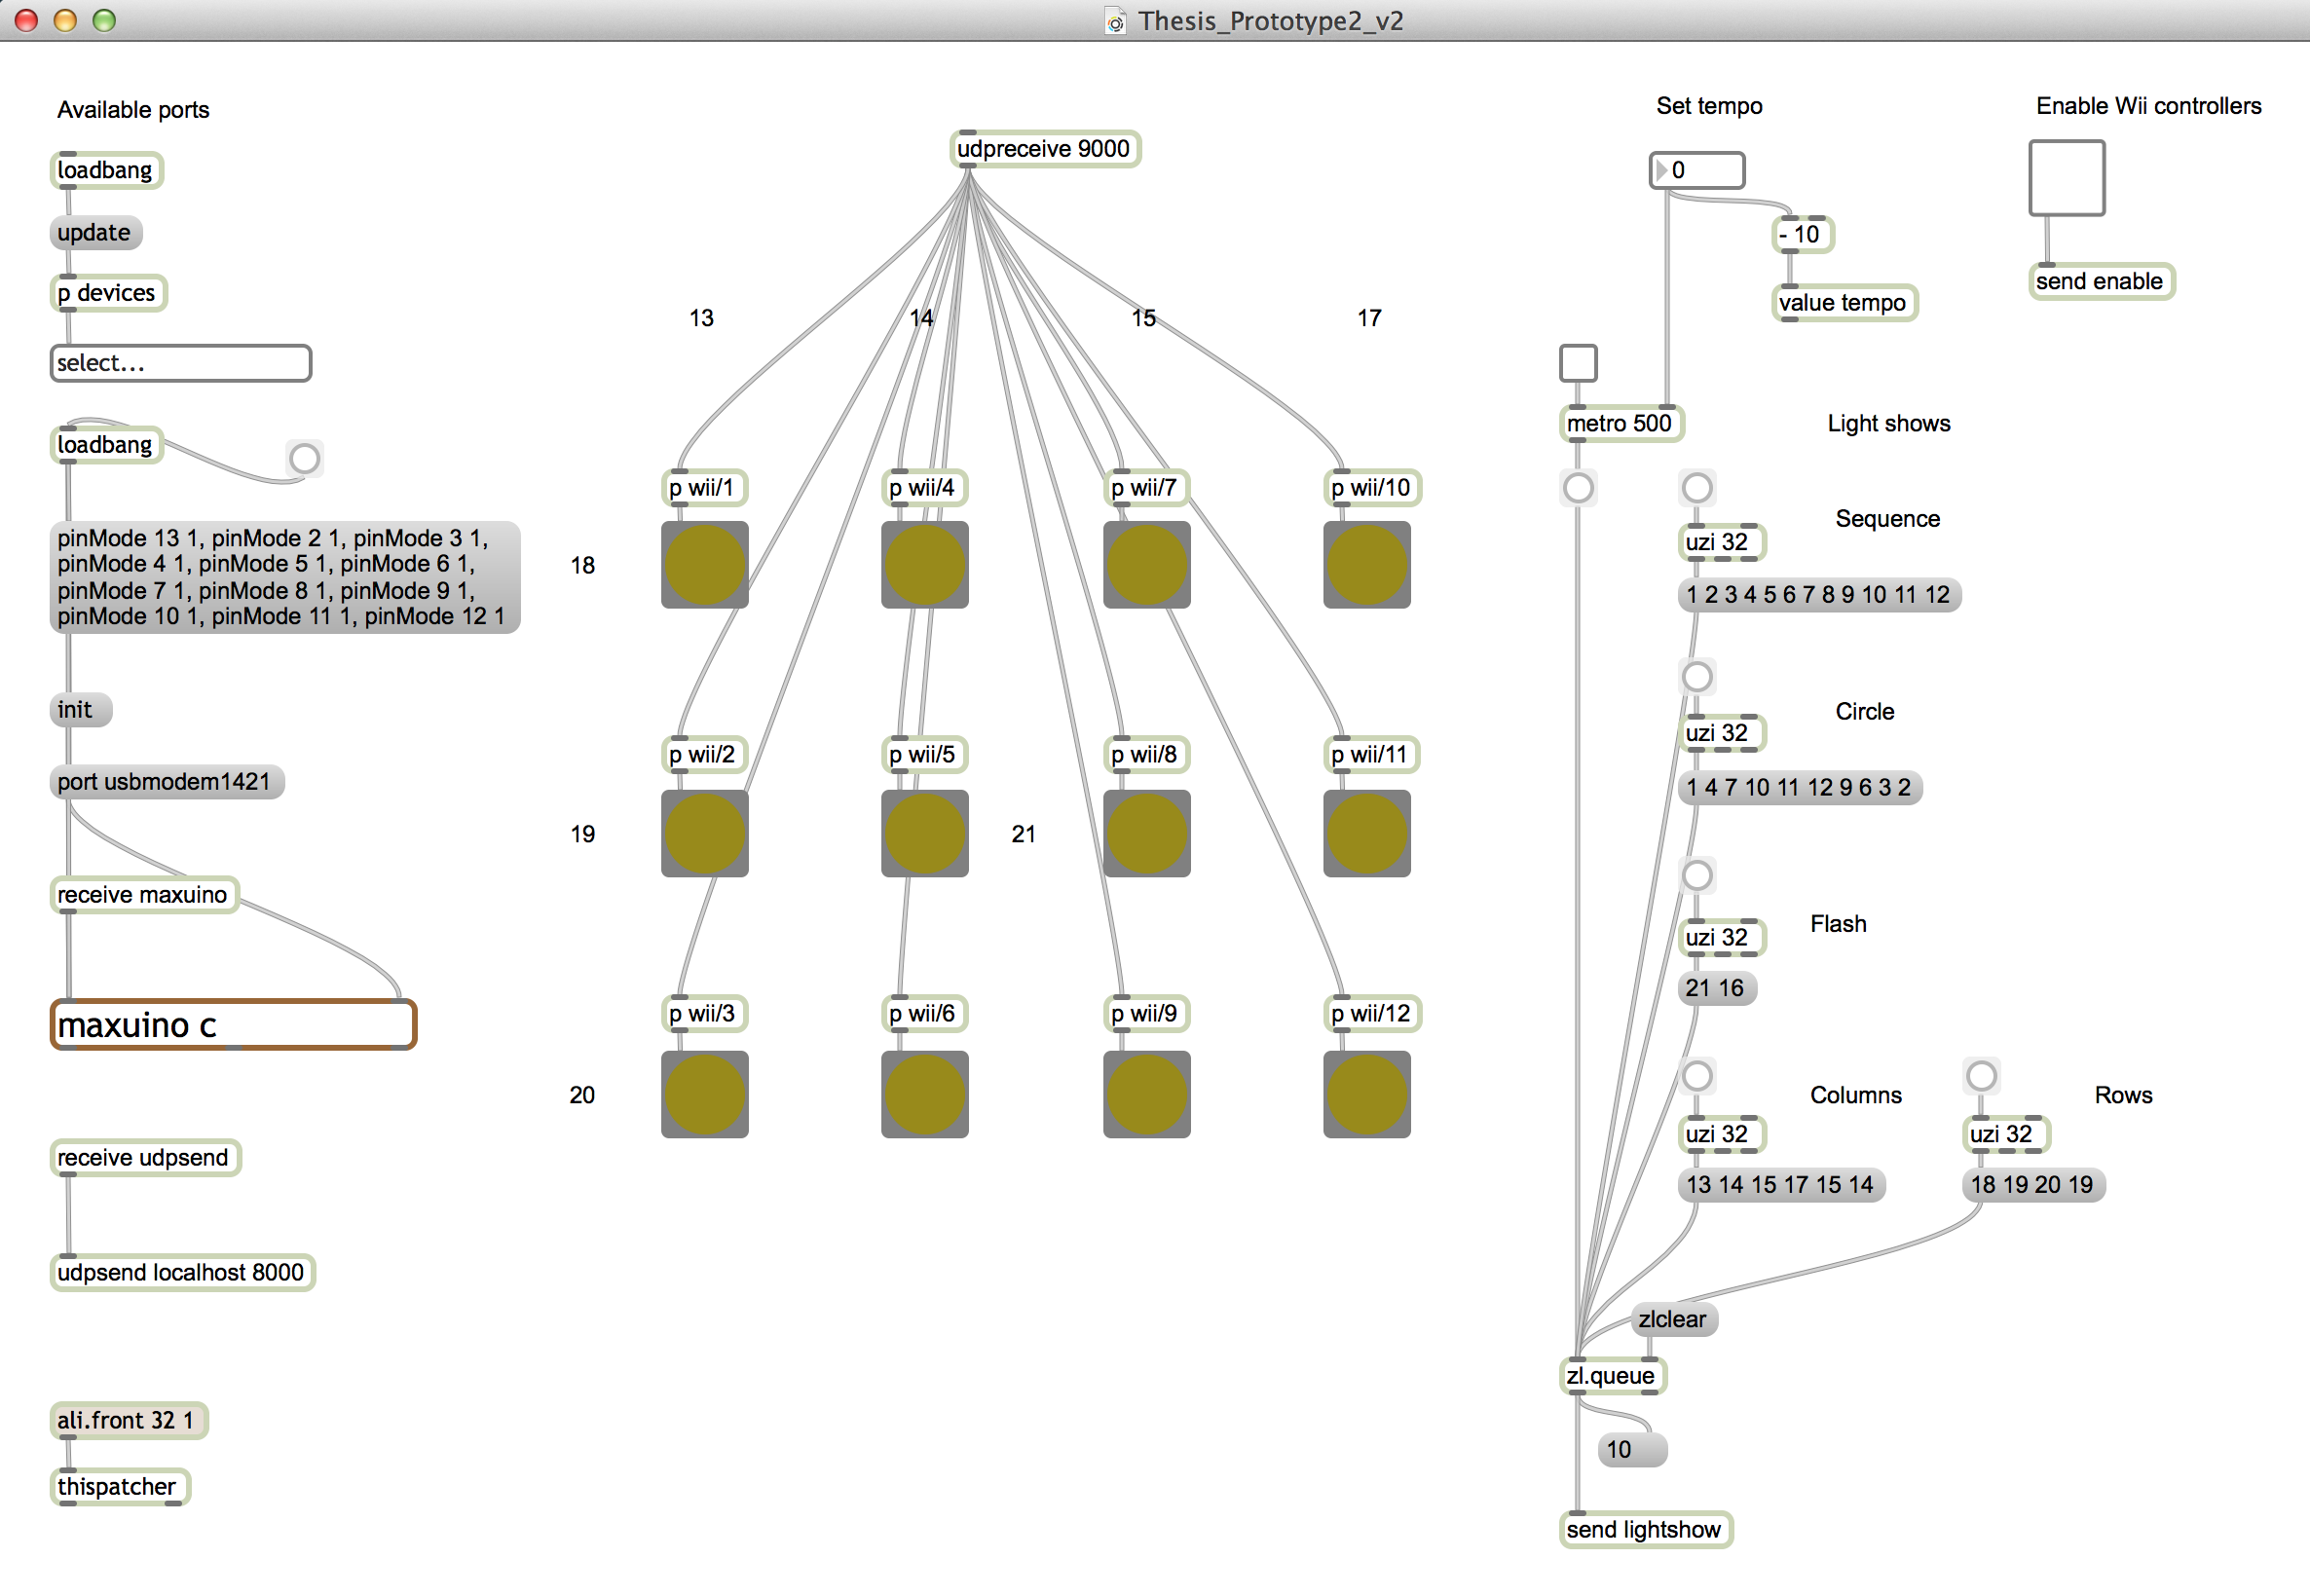
\includegraphics[height=0.4\textwidth]{control.png}
	\caption{Control and monitoring in Max}

	\label{prototyping3.6}
\end{figure}

Removed vibration feedback for interaction portion. The latency was too high, possibly confusing. Carefully fine-tuned the input sensitivity, bounce delay.

Made foam padding for Wii controllers to bury buttons. Taped up the controllers. Figure \ref{prototyping3.7}.

\begin{figure}[t]
	\centering

	\subfloat[Controller with foam cover]{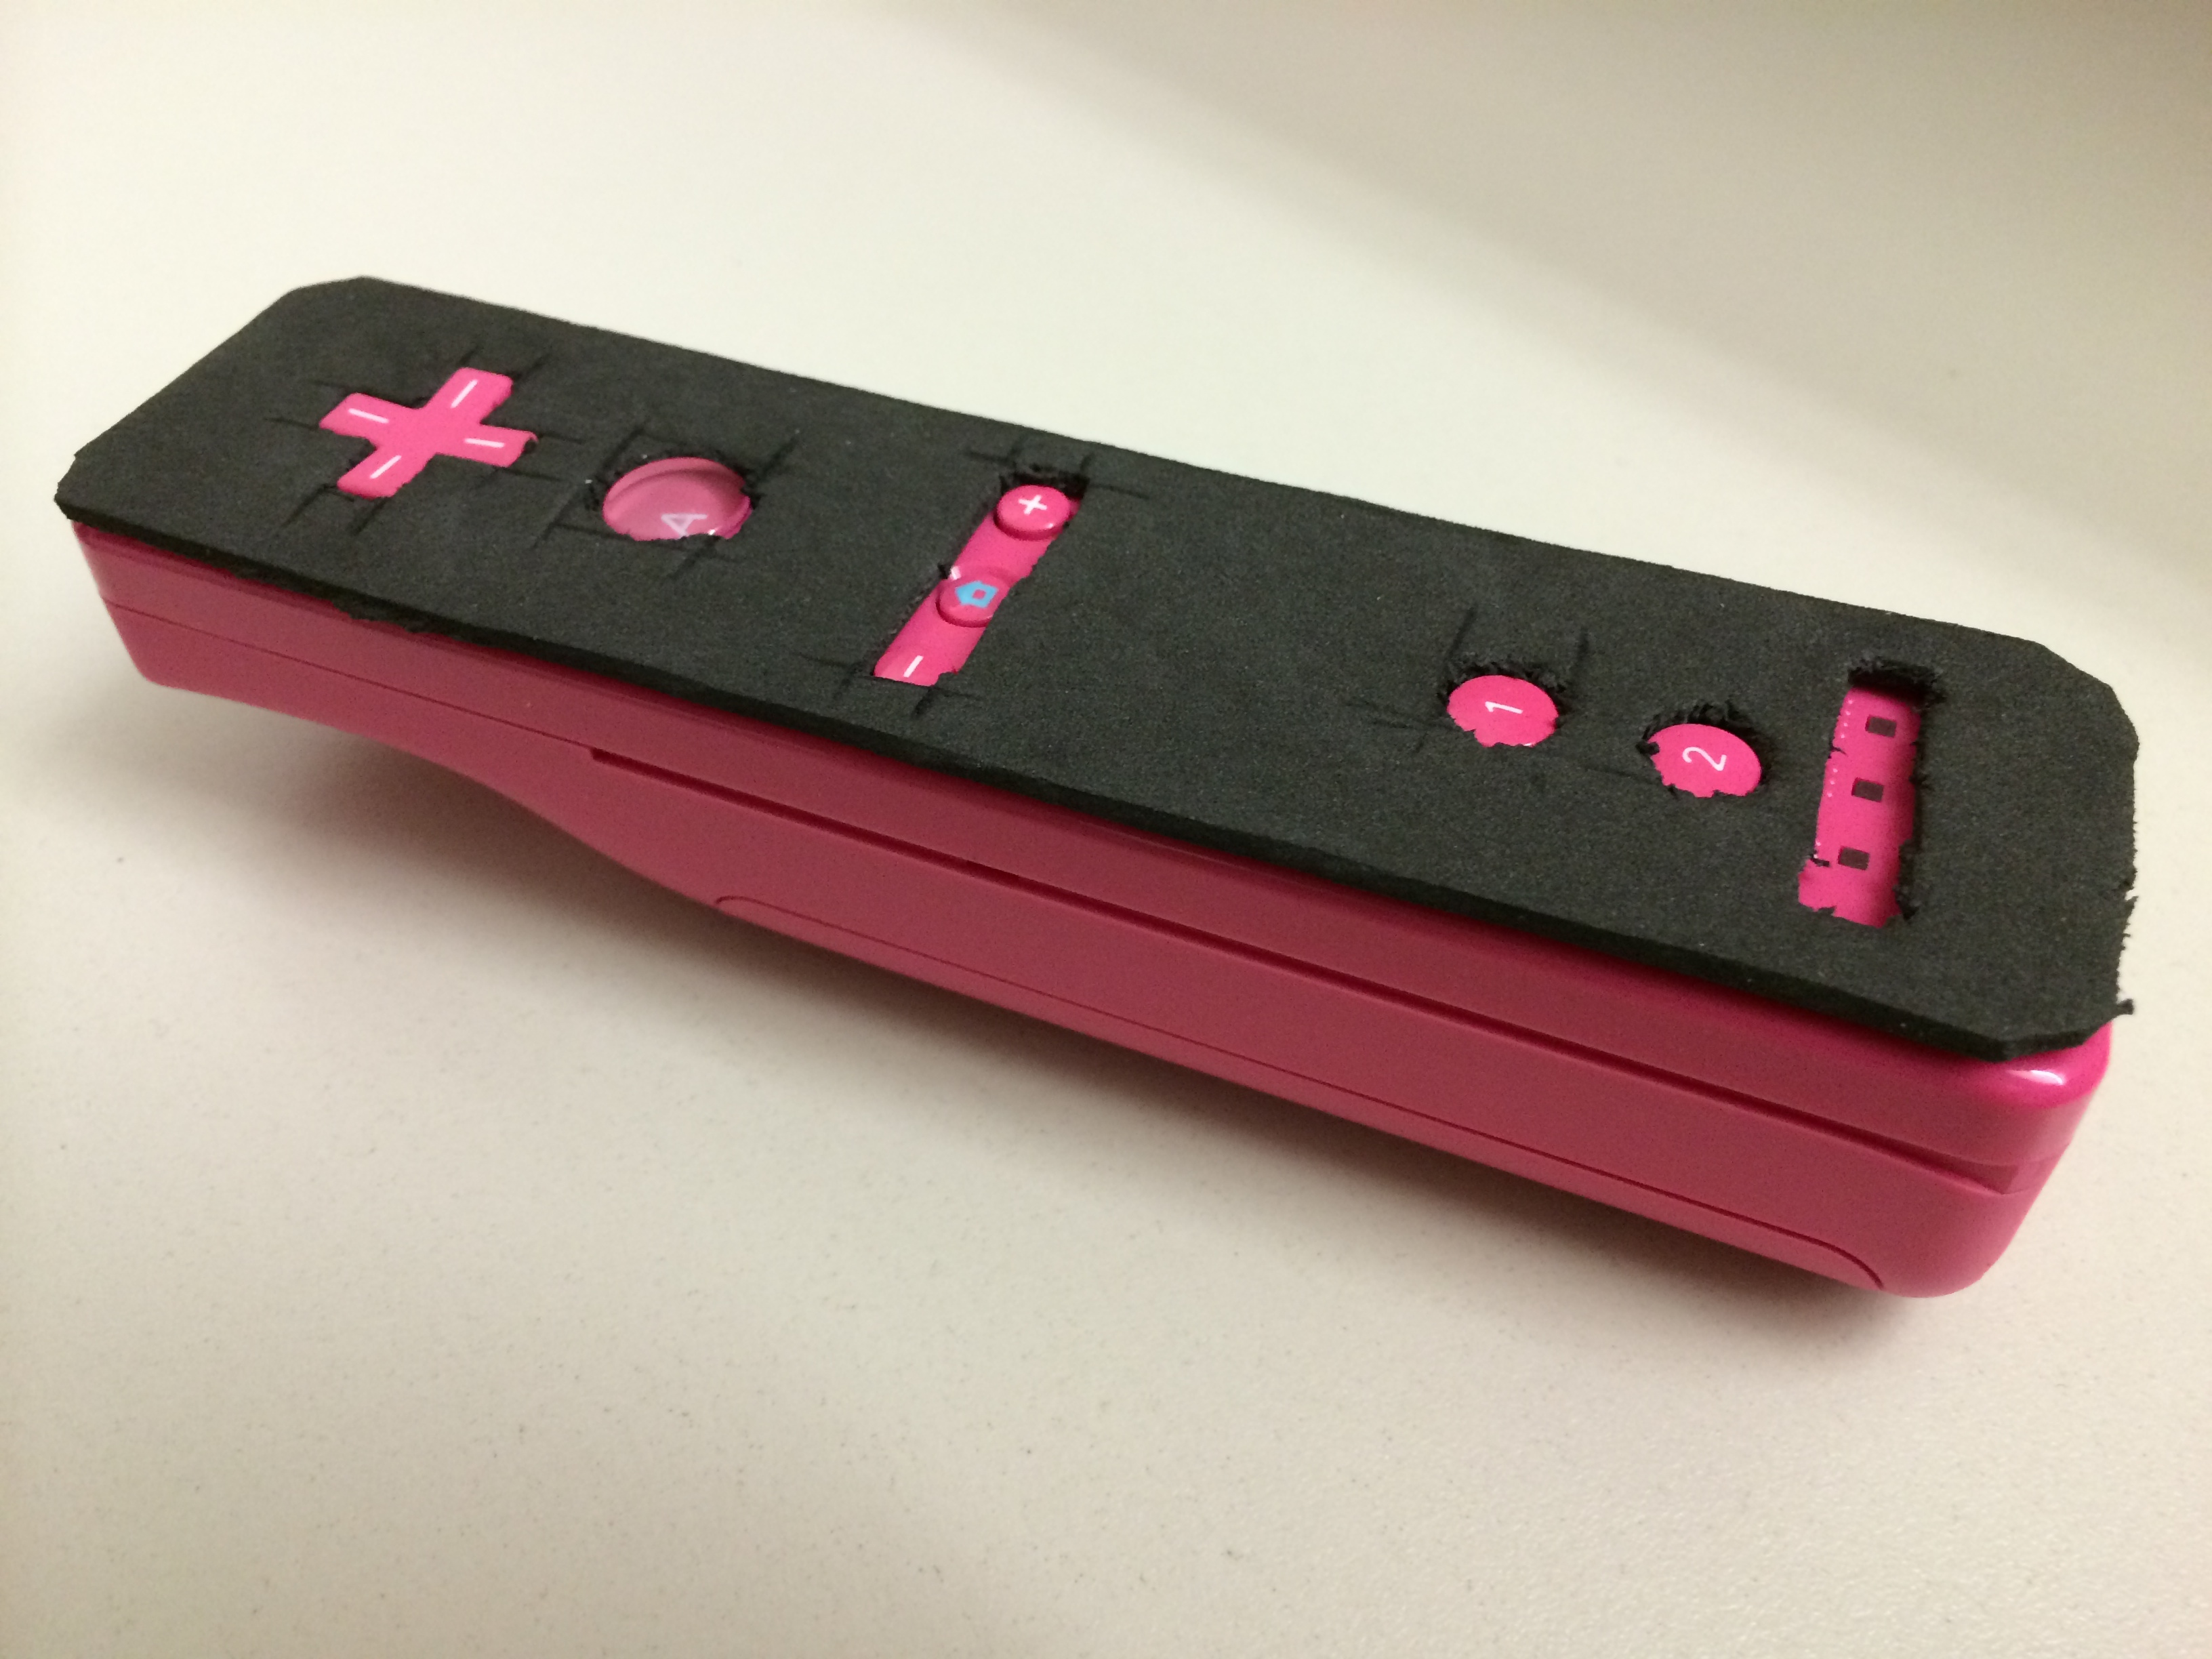
\includegraphics[height=0.36\textwidth]{wii.jpg}}
	\hspace{0.1cm}
	\subfloat[Taped controllers]{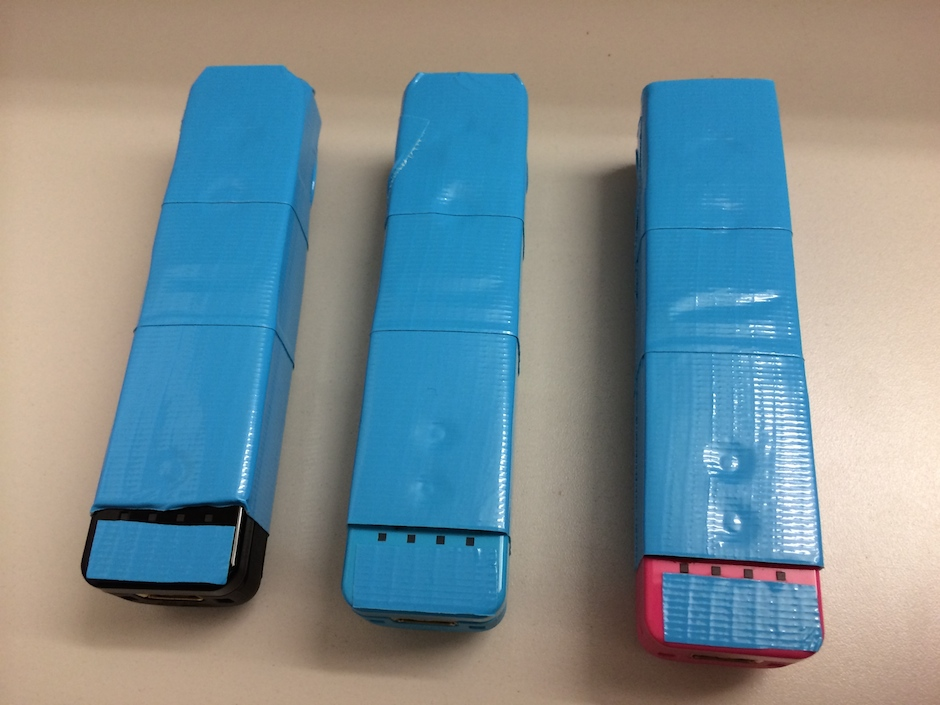
\includegraphics[height=0.36\textwidth]{wiis.jpg}}

	\caption{Preparing the Wii controllers}

	\label{prototyping3.7}
\end{figure}

\subsection{Testing}
% Explain the details of how participants were recruited, how data was collected, recorded, and processed/analyzed, and the timeline over which this process unfolded

The prototype was tested at a performance at The Silver Dollar Room. Figure \ref{prototyping3.8}.

\begin{figure}[t]
	\centering

	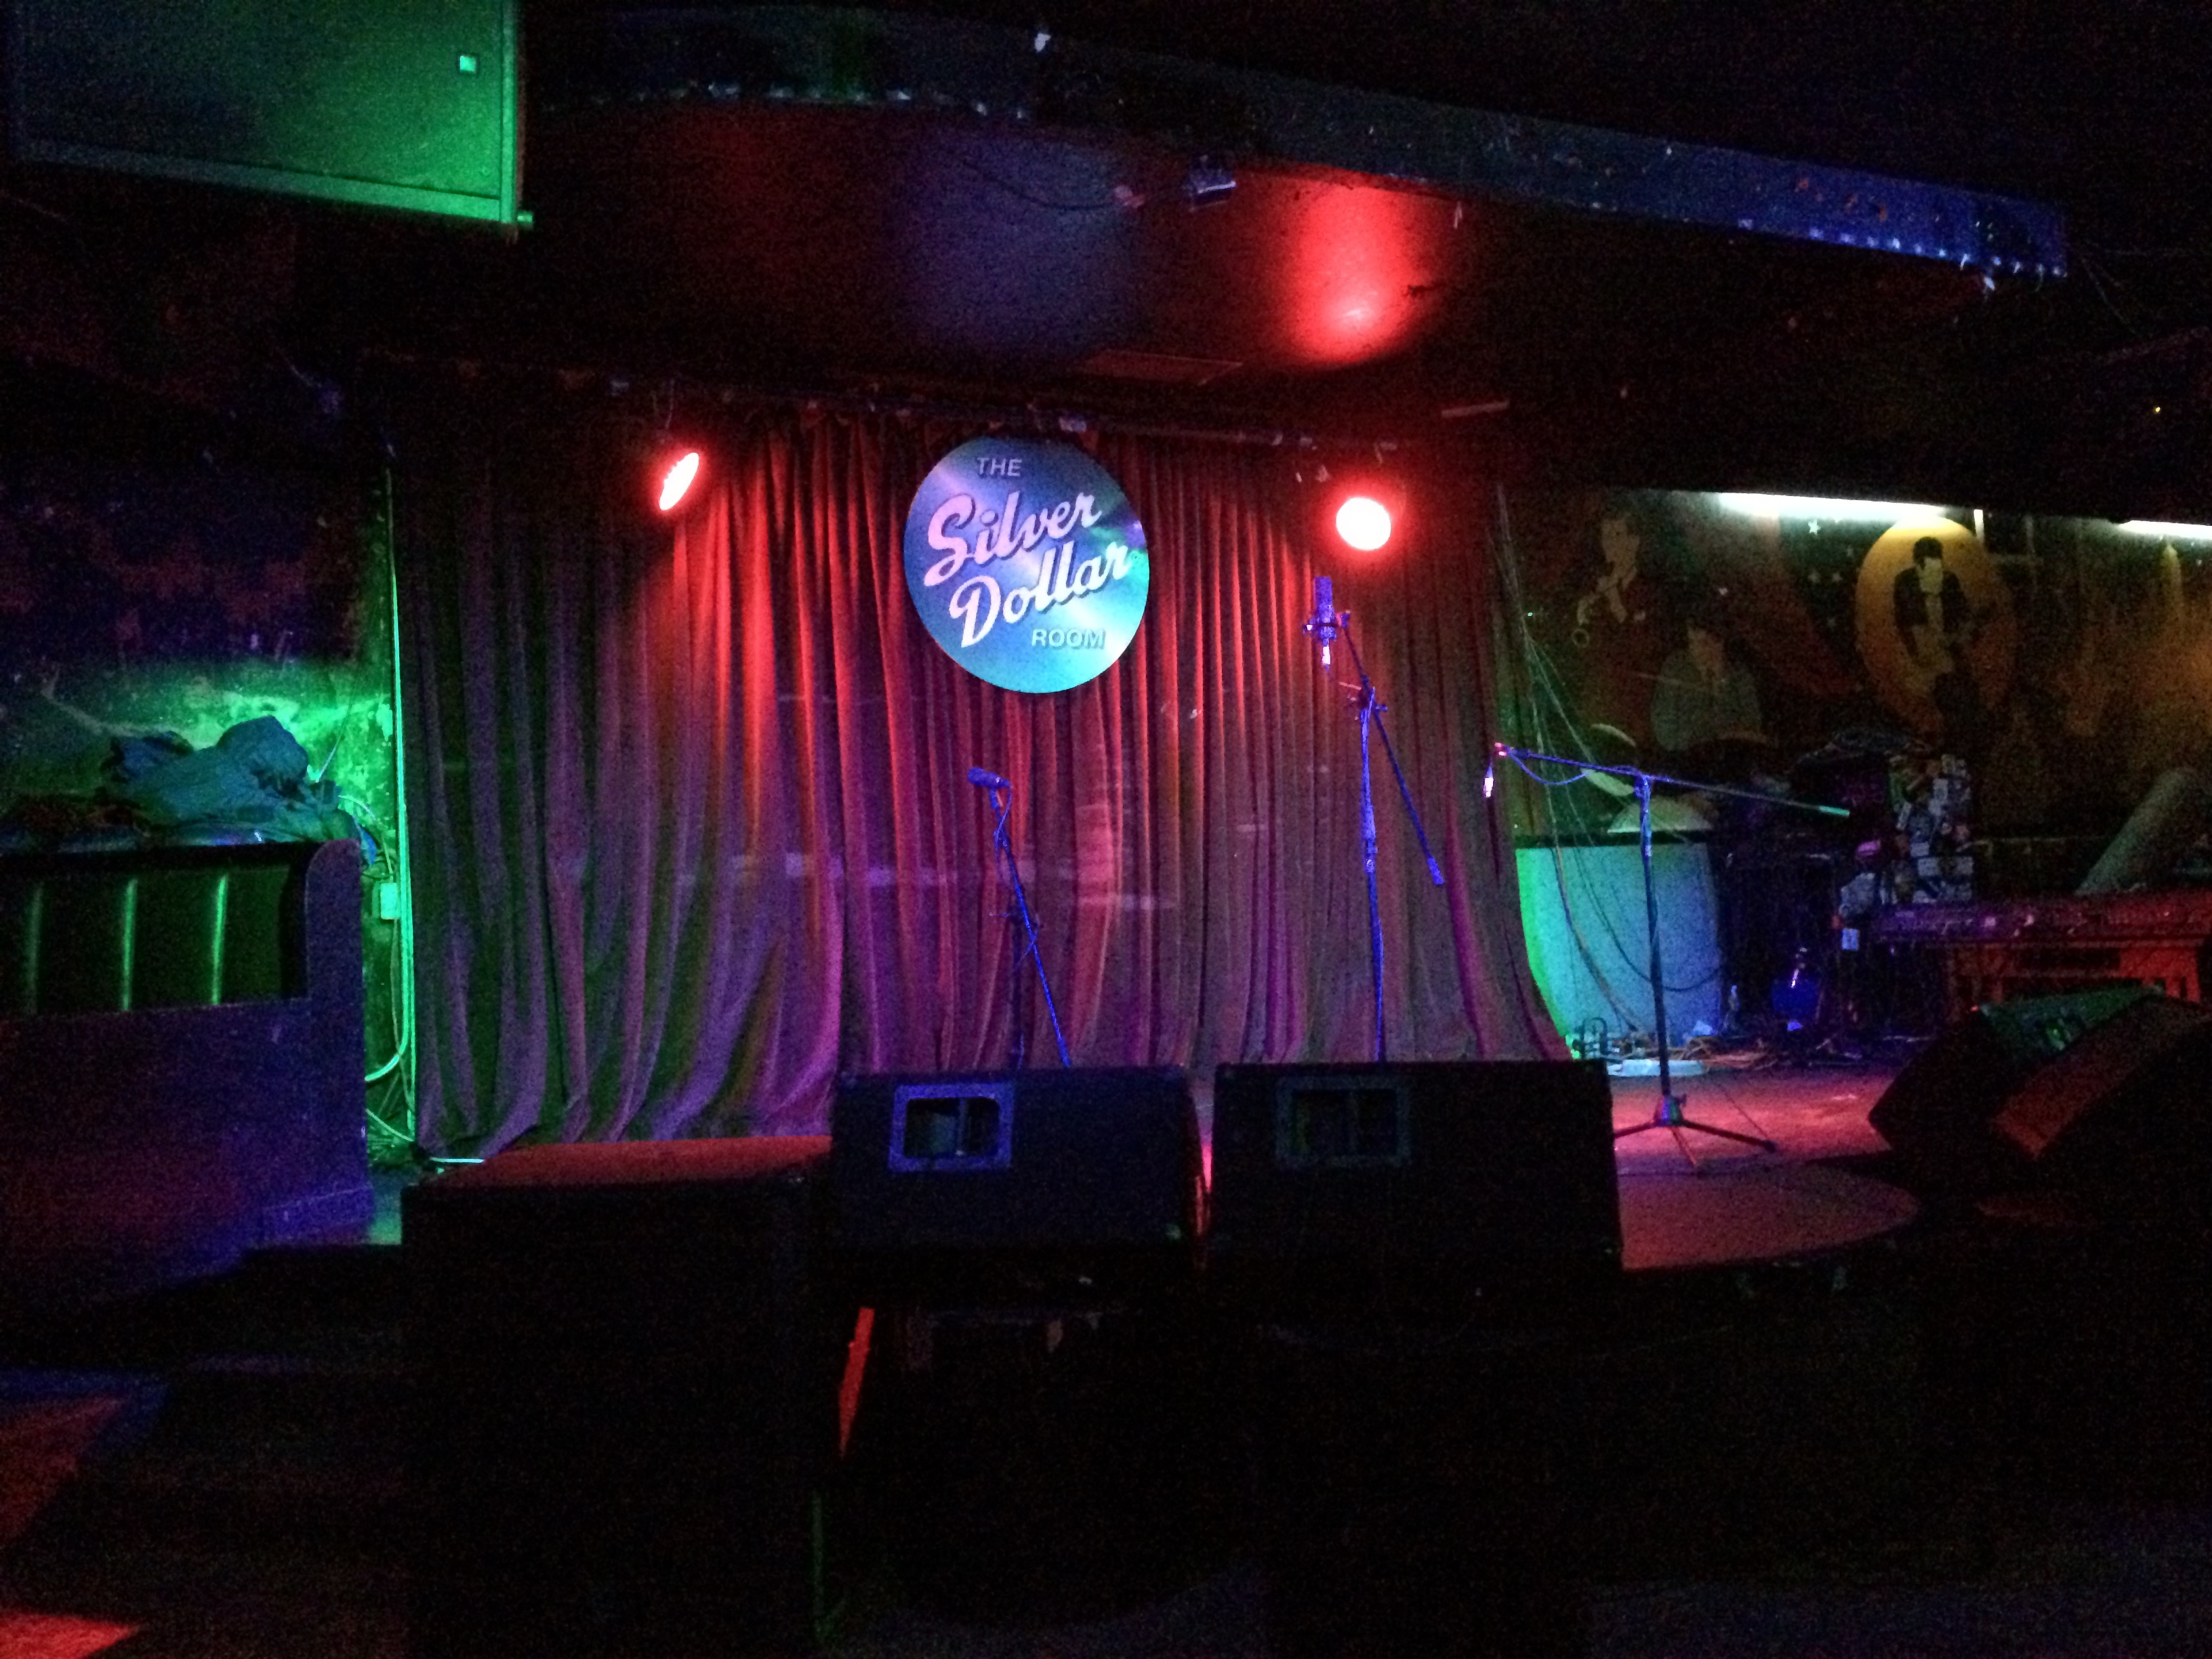
\includegraphics[height=0.4\textwidth]{silver_dollar.jpg}
	\caption{The Silver Dollar Room}

	\label{prototyping3.8}
\end{figure}

\subsubsection{Audience}

\subsubsection{Performers}

\subsection{Analysis}

% The obscure form of the device gave people options on how they'd like to use it

% Audience members did not make an attempt to work together. Was this due to attitude or size of the crowd? Or was this a limitation of the technology?
